\pdfoutput=1
\documentclass[10pt]{article}

\usepackage[preprint]{tmlr}

\usepackage{amsmath,amssymb}
\usepackage{graphicx}
\usepackage{booktabs}
\usepackage{longtable}
\usepackage{float}
\usepackage[colorlinks=true,linkcolor=blue,citecolor=blue,urlcolor=blue]{hyperref}


\newcommand{\R}{R}
\newcommand{\Sel}{S}
\newcommand{\G}{G}
\newcommand{\epsG}{\varepsilon_G}

\title{What a Linear-Probe Verdict Cannot Tell Apart: \\
A Measurement Audit of Self-Supervised Invariance}

\author{\name Ethan Hung \\
      \addr Independent Researcher}


\begin{document}
\maketitle

\begingroup
\renewcommand{\thefootnote}{\fnsymbol{footnote}}
\footnotetext[1]{\textbf{AI use disclosure.} Claude Sonnet 5 was used to document, revise
prose and organization, organize citations, assist with LaTeX, and check consistency between
manuscript claims and released artifacts. The author reviewed the resulting text, verified the
citations and numerical claims, and takes full responsibility for the paper.}
\endgroup

\begin{abstract}
Researchers call a self-supervised encoder invariant to a generative factor when a probe recovers it
poorly from the frozen representation. The inference assumes the augmentation manipulates the
intended factor and the probe can recover what the representation kept. In this work, we test both
assumptions. We train small SimCLR encoders on complete factorial grids (Shapes3D and dSprites; three
augmentation conditions, twelve seeds each) and fit four probe families to them and to a matched
untrained encoder. Before targeted-factor evaluation, two of five designed conditions were removed:
rotation, whose in-plane image transformation mismatches a bounded 3D camera-azimuth factor, and
scale, which failed a quality gate on object shape, where exploratory measurements suggest a color
shortcut in its single-augmentation recipe. Most importantly, we find that, on the three Shapes3D hue
factors, a closure statistic separates two augmentation regimes the thresholded linear-probe verdict
conflates: the deficit narrows across fitted probe families in the minimal-augmentation arm and widens
in the color arm (disjoint bootstrap intervals; one color-arm interval includes zero). We further show
that the linear rung's scores separate those arms by $0.714$ to $0.941$ of the normalized scale. Those
arms also apply disjoint augmentation sets, and we exempt the minimal-augmentation baseline from that
gate, which it fails on all twelve seeds. Finally, we show that a probe-free counterfactual
displacement statistic, calibrated on a fixture with known decodability and scored against an
untrained-encoder null, separates the same hue factors and arms by more than two orders of magnitude
before rank correction and by roughly twentyfold after it. For small SimCLR encoders on synthetic
factorial grids, we recommend an untargeted-factor check, probe families with a matched untrained
encoder, and paired displacement where exact counterfactuals exist.
\end{abstract}

\section{Introduction}
\label{sec:intro}
Linear probing is a common test of invariance in self-supervised representations: a probe is fitted
to a frozen encoder, and poor recovery of a generative factor is taken as evidence of invariance to
it. That interpretation relies on two assumptions. First, the
augmentation must manipulate the factor assigned to it. SimCLR makes this connection explicitly
\citep{chen2020simple}, while \citet{vonkugelgen2021self} show why image transformations can alter
latent factors in unexpected ways. Second, the probe must be capable of recovering the factor when
the representation retains it. Most natural-image studies cannot test these assumptions directly
because their latent factors and exact counterfactual pairs are unavailable.

Shapes3D and dSprites provide a controlled alternative. Both enumerate complete factorial grids,
with independently sampled factors known by construction. For any factor value and context, the grid
contains a corresponding image that changes only that factor, and that structure supports three
checks. A preserved-factor gate tests whether training damaged information outside the intended
target. A capacity ladder compares a linear probe with stronger probe families at a fixed training
sample size. Exact counterfactual pairs then measure the factor-induced displacement of the
representation directly, using a matched untrained encoder as the reference distribution.

We apply these checks to small SimCLR encoders trained on both datasets. The confirmatory design
contains three augmentation conditions with twelve seeds each, four probe families, and one fixed
probe-training budget. We removed two more conditions before targeted-factor evaluation, on two
different grounds (Section~\ref{sec:gate}). The study uses a ResNet-18 backbone, $64\times64$
synthetic images, one contrastive objective and one augmentation strength, so its conclusions
concern the validity of the measurement in that setting.

\begin{itemize}
\item \textbf{Correspondence audit.} A gate on object shape, an untargeted factor, identified two failures among
the five designed conditions before targeted-factor evaluation.
Rotation used a 2D $SO(2)$ transformation for a bounded 3D camera-azimuth factor. The
scale condition used whole-scene affine zoom in place of the preregistered random-resized crop, and
two exploratory measurements, a twelve-seed weak-color arm and a one-seed recipe pilot, suggest its
failure lies in the training recipe (Section~\ref{sec:gate}).

\item \textbf{Capacity dissociation.} For the three Shapes3D hue factors, the closure fraction
is positive in Control-aug, the minimal-augmentation baseline, and negative in the color arm,
with disjoint bootstrap intervals, one of which includes zero (Section~\ref{sec:kappa}). The
linear rung gives both arms the same $\epsilon$-invariance verdict while separating their scores
by $0.714$ to $0.941$ of the normalized scale. Across the ladder the deficit closes in the first
arm and widens in the second, which inverts the preregistered prediction. We read that ladder as
a fitted trajectory over probe families under one fixed training procedure, not as a limit of
mathematical capacity. The two arms apply disjoint augmentation
sets and differ in gate status, so we treat this as a difference between augmentation regimes.

\item \textbf{Probe-free displacement audit.} Counterfactual factor sweeps report whether a factor's
displacement falls below the calibrated band at the stated whitening rank. Raw displacement places
the two hue regimes more than
two orders of magnitude apart, and about twenty to twenty-three times apart once we correct for
their unlike whitening rank (Sections~\ref{sec:disp-results} and~\ref{sec:limitations}).
\end{itemize}

Random encoders already perform near the ceiling on these datasets, a property of the benchmarks
that prior work established. Prior studies recommend random-weight controls
\citep{saxe2011random}, report competitive untrained representations on Shapes3D and dSprites
\citep{cao2022empirical,maziarka2021relationship}, and find saturated in-distribution factor
prediction across many methods \citep{schott2022visual}. At our pinned configuration the deepest
probes on untrained encoders reach $0.976$ to $0.997$ for the targeted factors, leaving at most
$0.0243$ of normalized headroom, so the counterfactual statistic carries the positive claim.

We fixed the four hypotheses, their decision rules, and every operational definition on 2026-06-28,
before collecting data, and broke the blind on 2026-08-24. We chose this paper's organization after unblinding, so
Section~\ref{sec:prereg} reports all four preregistered verdicts under their frozen rules whatever
those rules returned. Appendix~\ref{app:amendments} records the fifteen dated amendments and their
unblinding status, and names the one change made after that trail ends: we filed the closure
fraction as a supporting diagnostic, and this paper organizes its results around it.

\section{Related Work}
\label{sec:related}

\subsection{Augmentations and learned invariance}
SimCLR links augmentation choice to the invariances acquired by an encoder
\citep{chen2020simple}. Later work examines view selection \citep{tian2020makes}, questions whether
complete invariance is desirable \citep{tamkin2022feature}, and analyzes contrastive objectives
spectrally \citep{haochen2021provable,balestriero2022contrastive}. Correspondence between an image
transform and a latent factor still requires care. \citet{vonkugelgen2021self} show that an
augmentation may affect unexpected ground-truth factors and report object hue surviving crop with
color distortion because of latent dependence. Independent factors in a complete grid let us test
that correspondence directly.

Projection heads provide another possible location for invariance. \citet{cosentino2022geometry}
find that much of the effect can concentrate in the projector, and \citet{chaudhry2026geometry}
model the head as a trainable metric on the backbone, attributing head-induced invariance to metric
degeneracy. We therefore evaluate the frozen backbone and report the projector separately in
Section~\ref{sec:h4}.

\subsection{Probe capacity and controls}
Probe conclusions depend on the predictor family. \citet{hewitt2019designing} favor constrained
probes and use random-label control tasks to quantify what the probe contributes.
\citet{pimentel2020information} instead interpret probing as a lower bound on mutual information,
which motivates expressive predictors. Related accounts formalize usable information
\citep{xu2020theory}, measure probe effort through description length \citep{voita2020information},
and review the selectivity and memorization problems of nonlinear probes
\citep{belinkov2022probing}.

Capacity sweeps offer a practical comparison across predictor families. Explicitness measures the
area under a loss-capacity curve \citep{eastwood2023dcies}; factor-prediction studies compare trees
and multilayer perceptrons \citep{dittadi2021transfer}; and \citet{rashtchian2023substance} evaluate
linear and nonlinear probes at several widths around the SimCLR projector. The affine-stable
hierarchy of \citet{lee2026shallow} gives linear probes a principled role and shows where quadratic
probes recover additional information. Our four-rung ladder is a simpler, parameter-count ordering,
so Section~\ref{sec:ladder} reports its optimization and monotonicity checks explicitly.

Random encoders provide the second control. \citet{saxe2011random} recommend separating
architectural effects from learning through random-weight performance. On dSprites,
\citet{cao2022empirical} find a high FactorVAE score for a randomly initialized representation.
\citet{maziarka2021relationship} report similarly strong untrained DCI informativeness on Shapes3D,
and \citet{schott2022visual} observe near-ceiling in-distribution factor prediction across seventeen
methods. These findings motivate our matched random-encoder floor and per-factor headroom analysis.
Our broader experimental design follows the controlled comparison principles of
\citet{locatello2019challenging}.

The capacity effect in our minimal-augmentation arm resembles linear concept erasure in reverse.
Closed-form erasure can make a concept inaccessible to every linear classifier while preserving it
for nonlinear recovery \citep{belrose2023leace}; amnesic probing provides an intervention-based
variant \citep{elazar2021amnesic}. Our fitted linear probe offers a weaker test, so we use the
descriptive term ``present but linearly inaccessible.'' \citet{foster2021probing} report transform
parameters that remain linearly recoverable in nominally invariant representations. That is the
nearest published comparison for this regime.

\subsection{Probe-free invariance measures}
Frozen-feature invariance tests predate modern self-supervised learning
\citep{goodfellow2009measuring}. Interventional robustness scores later used factorial datasets to
hold one factor fixed while varying the others \citep{suter2019robustly}. We reverse that operation
by changing the target factor at a fixed context. The resulting statistic is a whitened
displacement,
related to the Mahalanobis measurements of \citet{ericsson2022why} and the unwhitened alignment term
of \citet{wang2020understanding}.

Recent probe-free methods address complementary parts of the problem. SEIS uses CCA on denoised
activation subspaces to separate invariance from equivariance \citep{lin2026seis}. EditCLEVR changes
one object attribute at a time and reports localization and drift measures alongside decoded
semantics \citep{karnam2026editclevr}. SEIS scores against a random baseline on a relative
scale, and EditCLEVR compares paired scenes without a matched untrained-encoder null. The complete
grid used here
supports repeated contexts, an untrained null, an absolute calibration band, and a decomposition of
shared and context-dependent displacement. We cite the 2026 works in this discussion
\citep{lee2026shallow,lin2026seis,karnam2026editclevr,chaudhry2026geometry} from their arXiv
versions. \citet{chaudhry2026geometry} is listed there as accepted at ICML 2026.

\subsection{Measurement gap}
\label{sec:positioning}
The unresolved question is whether a linear-probe invariance verdict distinguishes representational
states that behave differently under stronger probes and direct counterfactual tests. Our design combines independent factorial sampling, a capacity ladder, a random-label control, a
matched untrained encoder and calibrated counterfactual displacement, so it tests correspondence
and probe sufficiency together within the stated small-model, synthetic-data setting.

The probe-side instruments come from prior work. Our ladder is the explicitness sweep of
\citet{eastwood2023dcies}, the control task is \citet{hewitt2019designing}'s, and the observation
that a nonlinear probe recovers what a linear one misses is established across domains. What is new
here is the contrast they are put to: two closure regimes on matched factors, at twelve seeds,
against one shared untrained-encoder array, inside a controlled invariance measurement on small
SimCLR encoders and synthetic grids.

\section{Problem Setup: What an Invariance Verdict Assumes}
\label{sec:defs}

\subsection{Generative factors and ground truth}
Both datasets are complete factorial grids with exact generative-factor labels. Shapes3D supplies
floor, wall and object hue at ten values each, scale at
eight, orientation at fifteen and shape at four, giving $480{,}000$ images at $64\times64$. We treat
five of those as continuous and shape as categorical. dSprites supplies shape at three values,
scale at six, orientation at forty, and $x$ and $y$ position at thirty-two each.

Orientation differs between the two datasets. Shapes3D orientation is a bounded arc of 3D camera
azimuth, while dSprites orientation is the full circle, and because the square is
$90^\circ$-periodic and the ellipse $180^\circ$-periodic, distinct latent orientations there map to
identical images. Pixel-level non-identifiability excludes this readout from the confirmatory families. It remains in the diagnostic results.

Independent sampling has two consequences. When pairs that differ in one factor map to the same
representation, the representation becomes a function of the remaining factors, preventing recovery
of the changed factor at any probe capacity. Independence also removes the latent-dependence account
used by \citet{vonkugelgen2021self} for surviving hue. A shortcut through another factor remains
possible: Section~\ref{sec:gate} shows that hue alone can solve NT-Xent on this grid because of its
cardinality and the benchmark construction.

\subsection{Recoverability, selectivity, and encoder gain}
Write $h = f(x) \in \mathbb{R}^{512}$ for the frozen backbone representation, $F$ for a generative
factor and $c$ for probe capacity. All three quantities below are measured on a held-out probe-test split.
Table~\ref{tab:notation} in Appendix~\ref{app:notation} collects every symbol this paper uses
alongside the conditions under which it becomes undefined.
\textbf{Recoverability} is probe-test performance predicting $F$ from $h$, normalized per factor
type:
\begin{equation}
\R(F, c) =
\begin{cases}
\dfrac{\mathrm{acc}(F,c) - \mathrm{acc}_{\mathrm{chance}}(F)}{1 - \mathrm{acc}_{\mathrm{chance}}(F)}
  & F \text{ categorical},\\[1.8ex]
R^2(F, c) & F \text{ continuous},
\end{cases}
\qquad
\Sel(F, c) = \R(F, c) - \R^{\mathrm{perm}}(F, c).
\label{eq:RS}
\end{equation}
We retain negative $R^2$ because clipping would bias encoder gain upward.
\textbf{Selectivity} $\Sel$ is the control task of \citet{hewitt2019designing}, and it bounds the
\emph{probe}. Our $\R^{\mathrm{perm}}$ uses a value-to-target permutation applied identically across
splits, so the permuted label stays a function of the image and a high-capacity probe genuinely can
fit it. A selectivity near zero therefore indicates that the probe is memorizing. Under this
construction $\Sel \equiv 0$ for categorical factors, and every targeted factor here is continuous.
\textbf{Encoder gain} is our preregistered headline metric. It bounds \emph{representation-free}
structure by
subtracting a matched-architecture untrained encoder, and the \textbf{capacity gap} differences the
top rung against the linear one:
\begin{equation}
\G(F, c) \;=\; \R^{\mathrm{trained}}(F, c) - \R^{\mathrm{random}}(F, c),
\qquad
\Delta_{\G}(F) \;=\; \G(F, c_4) - \G(F, c_1).
\label{eq:G}
\end{equation}
A random-encoder floor near the ceiling compresses $\G$ toward zero. We therefore co-report the
headroom-normalized quantity $\tilde{\G} = \G / (1 - \R^{\mathrm{random}})$. Normalized accuracy and
$R^2$ use different units. Each value of $\G$ is interpreted against its factor-specific threshold,
and cross-factor comparisons are restricted to factors of the same type, a restriction whose effect
on the preregistered prediction Section~\ref{sec:limitations} explains.


\subsection{\texorpdfstring{$\epsG$}{epsilon-G}-invariance, the dual gate, and the closure fraction}
\label{sec:closuredef}
Let $\epsG(F)$ be the $97.5$th percentile of the factor-specific gain distribution under a
random-versus-random encoder null, estimated with the paired seed bootstrap used throughout. We
also report a fixed $\epsG = 0.05$ sensitivity analysis. Three cases exhaust the decision rule:
$\G \le \epsG$ is $\epsilon$-invariance, with $\G < 0$ reported separately; $\G > \epsG$ and
$\Sel > 0$ is genuine recovery; and $\G > \epsG$ with $\Sel \le 0$ is inconclusive and
probe-driven. Here, $\epsilon$-invariance means that encoder gain was below the detection threshold.
Absolute trained performance, the random floor, and projector performance accompany each decision
so that saturation remains visible.

Our primary decision is two-sided. Define the deficit as $D(F,c) = \R^{\mathrm{random}}(F,c) -
\R^{\mathrm{trained}}(F,c) = -\G(F,c)$ and let $\epsilon_D$ be the corresponding percentile in the
deficit direction. A readout is \emph{suppressed} when $D > \epsilon_D$ and \emph{recovered}
otherwise. Suppression at every rung gives $\epsilon$-invariance. The flip count records readouts
that are suppressed at the linear rung and recovered at the top. Values at the untrained floor are
classified as recovered, since genuine invariance requires training to push recoverability below
that floor. Because the null pool is symmetric, $\epsilon_D = \epsG$ numerically. We retain the
frozen
one-sided rule as a sensitivity analysis.

A \textbf{null-saturation gate} removes a readout from the genuine-invariance decision and flip
count
when its random-encoder floor reaches $0.90$ at either endpoint of the ladder, though such readouts
remain available as diagnostics. At this ceiling, $\G \le \epsG$ conflates suppression with limited
headroom above the architectural prior. Differencing the two probe endpoints leaves the capacity gap
unaffected.

The \textbf{closure fraction} summarizes the recoverability-versus-capacity curve in one number:
\begin{equation}
\kappa(F) \;=\; 1 \;-\; \frac{D(F, c_4)}{D(F, c_1)},
\qquad\text{defined only where } D(F, c_1) > 0.
\label{eq:kappa}
\end{equation}
A $\kappa$ near $+1$ indicates that the linear deficit closes across fitted probe families, consistent
with the regime formalized by \citet{belrose2023leace} as present but linearly inaccessible. Values
near $0$ indicate persistence, while negative values indicate a widening deficit. This statistic
measures suppression relative to the untrained floor. The probe-free analysis in
Section~\ref{sec:certificate} tests whether displacement falls below the calibrated band at the
stated whitening rank. The ratio is undefined
when the linear-rung deficit is nonpositive, and those cells are listed separately. Because negative
$R^2$ is retained, $D$ can exceed the width of the normalized scale. We therefore interpret
$\kappa$ as a shape statistic for the deficit curve, with both arguments shown in
Figure~\ref{fig:plane}.

Headroom-normalized gain $\tilde{\G}$ corrects the upper compression of $\G$ as $1 -
\R^{\mathrm{random}}$ approaches zero. The deficit has no analogous upper bound because
negative $R^2$ is retained. Consequently $\kappa$ is not headroom-normalized, and
Appendix~\ref{app:probebuild} evaluates two candidate renormalizations.

All three Shapes3D arms use the same untrained-encoder array for each seed, factor and probe rung,
so that shared floor cancels when capacity gaps are differenced between arms. The observed
separation comes from the trained representations. Section~\ref{sec:gap} reports their absolute
levels, disjoint twelve-seed ranges and the three between-arm differences, all of which survive
saturation, and we interpret the closure fraction alongside these floor-free comparisons.

\section{Method}
\label{sec:method}

\subsection{Encoders and augmentation conditions}
Each cell trains a SimCLR encoder \citep{chen2020simple}: a ResNet-18 backbone in the CIFAR variant
(512-dimensional $h$), a projector to 128 dimensions, NT-Xent at temperature $0.5$, 150{,}000 images
from a 400{,}000-image unlabeled split, batch 512, 50 epochs with 5 warmup, Adam at $10^{-3}$ and
weight decay $10^{-6}$.
The crop-plus-color arm is the one exception and ran 100 epochs.
Section~\ref{sec:limitations} discusses that difference.

Color and Control-aug reach comparable final NT-Xent and uniformity, which is what the
between-arm comparison of Section~\ref{sec:kappa} needs. Position and crop-plus-color optimize
differently and are unsuitable for matched-optimization comparisons with that pair, and Appendix~\ref{app:training} reports the per-arm
diagnostics.


Each condition applies an augmentation intended to change its assigned factor while limiting other
changes. Our three realized conditions are \textbf{color}, strong jitter with grayscale;
\textbf{position}, affine translation; and \textbf{Control-aug}, a random-resized crop alone. Two
designed conditions obtained no gate-passing encoder, \textbf{orientation} and \textbf{scale}, and
we excluded both before targeted-factor evaluation. Scale failed the preserved-shape gate of
Section~\ref{sec:controls}. We excluded orientation under the gate as it then stood and on a
preregistered group-action argument filed with the same decision, which is the ground that survives
a later revision of the gate (Section~\ref{sec:gate}).

We then froze the realized confirmatory grid at three cells. Three exploratory arms are reported
separately: \textbf{weak color}, at one quarter of the jitter with no grayscale and otherwise
identical to the strong color arm; \textbf{scale-recipe}, the same zoom composed with a photometric
base; and a crop composed with color jitter, introduced in Section~\ref{sec:limitations}. None
enters a confirmatory family or any multiple-comparison correction. Table~\ref{tab:conditions} lists
every transform as realized.

\begin{table}[t]
\centering
\caption{Realized augmentation compositions. Color, Position, and Control-aug form the confirmatory
grid; superscript e marks exploratory cells and superscript x marks exclusions made before
targeted-factor evaluation. Color and Control-aug share no transform, so their comparison is between
augmentation regimes (Sections~\ref{sec:kappa} and~\ref{sec:limitations}).}
\label{tab:conditions}
\small
\setlength{\tabcolsep}{3.5pt}
\begin{tabular}{l ccccc l l}
\toprule
 & \multicolumn{5}{c}{transform applied} & & \\
\cmidrule(lr){2-6}
Condition & crop & jitter & gray & translate & zoom/rot. & Targeted factor(s) & Also perturbs \\
\midrule
Color, strong        & --      & strong & yes & --   & --       & floor/wall/object hue & none \\
Color, weak \textsuperscript{e} & --      & weak   & --  & --   & --       & floor/wall/object hue & none \\
Position              & --      & --     & --  & 25\% & --       & $x$, $y$ position     & scale, aspect \\
Control-aug           & 0.8--1.0 & --     & --  & --   & --       & none (baseline)       & position, scale \\
\midrule
Orientation \textsuperscript{x}  & --      & --     & --  & --   & rot.\ $\pm30^\circ$ & orientation & apparent scale \\
Scale \textsuperscript{x}        & --      & --     & --  & --   & zoom 0.75--1.25 & scale & position \\
Scale + recipe \textsuperscript{e} & --    & mid    & yes & --   & zoom 0.75--1.25 & scale & position \\
Crop+color \textsuperscript{e} & 0.3--1.0 & mid & yes & -- & flip & floor/wall/object hue & position, scale \\
\bottomrule
\end{tabular}
\\[2pt]
{\footnotesize \textsuperscript{e} exploratory, in no confirmatory family. \textsuperscript{x}
excluded before any targeted-factor verdict, Scale on the encoder-quality gate and Orientation on
the group-action argument (Section~\ref{sec:gate}). Transforms as realized: strong jitter,
\texttt{ColorJitter(0.8,0.8,0.8,0.5)} at $p=0.8$ with \texttt{RandomGrayscale(0.2)}; weak jitter,
\texttt{ColorJitter(0.2,0.2,0.2,0.1)} at $p=0.8$, no grayscale; mid jitter,
\texttt{ColorJitter(0.4,0.4,0.4,0.1)} at $p=0.8$ with \texttt{RandomGrayscale(0.2)}; translate,
\texttt{RandomAffine} to $25\%$, rotation and scale fixed; crop,
\texttt{RandomResizedCrop(64, scale=(0.8,1.0))}; rot., \texttt{RandomRotation($\pm30^\circ$)};
zoom, \texttt{RandomAffine(scale=(0.75,1.25))}.}
\end{table}

\subsection{Probe-capacity ladder}
\label{sec:ladder}
Four probe families evaluate the frozen representation: \texttt{linear} ($512 \rightarrow
\text{out}$),
\texttt{mlp\_small} ($512 \rightarrow 64$), \texttt{mlp\_large} ($512 \rightarrow 256$) and
\texttt{mlp\_deep} ($512 \rightarrow 256 \rightarrow 128$). We report capacity as the trainable
parameter count per rung, which for a scalar target is $513$, $32{,}897$, $131{,}585$ and
$164{,}353$.

As \emph{function classes} the rungs nest, so parameter count orders a real inclusion chain of
hypothesis classes. Appendix~\ref{app:probebuild} gives the construction.

Fitted estimates depart from that ordering. Across the three confirmatory cells, $207$ of
$1{,}008$ rung-to-rung steps in the trained and random roles decrease. Those departures are largest in
the color arm, where trained recoverability falls on $20$, $21$ and $28$ of the $36$ steps for its
three hue factors, with a maximum drop of $0.157$, against $4$ of $216$ trained-role steps in
Control-aug. These declines produce the negative closure fractions of Section~\ref{sec:kappa}. Each
rung's estimate is the joint product of a probe family and the fixed training procedure we apply to
it, so a decline measures that pair and not a loss of information to a class that contains its
predecessor exactly. Every quantity we build on the ladder therefore describes a fitted-probe
trajectory rather than a capacity limit. This construction also lacks the affine invariance
established by \citet{lee2026shallow} for their shallow hierarchy.

We estimate optimization error by comparing two implementations of the linear probe, which differ
by $0.079$ on the random encoder's shape readout. Because the capacity gap differences the linear
rung against the top, an optimizer-limited linear rung inflates it, so we report every capacity gap
with an upper bias in the confirming direction of $+0.0099$ on Shapes3D and $+0.0113$ on dSprites,
closing to about $0.001$ at four times the budget. That linear rung also sits in the denominator of
$\kappa$, where the same budget moves the statistic by at most $0.014$ on thirteen of the fourteen
readouts where $\kappa$ is defined and leaves the dissociation intact. Control-aug shape is the
exception, and we report that readout as unresolvable on this instrument.
Appendix~\ref{app:probebuild} gives the rung-uniform weight-decay budget, whose selected values we
did not retain, with the per-role step counts and both sensitivity calculations.

\subsection{Controls and the encoder-quality gate}
\label{sec:controls}
The \textbf{random-label control} defines selectivity and bounds probe memorization. The
\textbf{random-encoder control} uses the same architecture, splits, probe ladder, and configuration
to estimate structure supplied by the architecture. A \textbf{supervised reference} provides a
recoverability ceiling, and a \textbf{raw-pixel reference ladder} is a diagnostic. We keep
those last two outside every decision rule.

Our \textbf{encoder-quality gate} checks representation quality before targeted-factor evaluation.
It requires both linear-rung shape recoverability at or above $0.90$ and shape
recoverability above the random-encoder floor by a margin of $0.02$. Shape is the preserved anchor. Every condition in the study leaves it untargeted, so the gate is
orthogonal to every targeted-factor hypothesis. We built the gate with three outcomes. An arm that
clears both thresholds passes. A closing shape deficit yields an indeterminate result and retains
the arm because it is consistent with limited linear access. A persistent deficit is the failure
branch and permits exclusion.

Control-aug is exempt because its role as the minimal-augmentation baseline makes
near-random shape recoverability expected. Under the same numerical rule it passes on $0$ of $12$
seeds: its anchor is $0.7370$, below the untrained floor of $0.7890$, and its shape deficit persists
across the ladder at
$0.052$, $0.055$, $0.054$ and $0.058$. That is the branch on which we excluded the scale arm. We
filed the exemption in amendment A2 on 2026-07-14, before either exclusion and before any
targeted-factor result, based on the baseline's preregistered design role. Our central comparison in
Section~\ref{sec:kappa} therefore pairs a gate-passing arm with an exempt arm, and
Section~\ref{sec:limitations} summarizes the evidence on encoder quality.

\subsection{Counterfactual displacement at a calibrated resolution}
\label{sec:certificate}
Because the grid is complete and its factors independent, a factor's effect on the representation
can be measured with no probe at all. Fix a context $z_{-F}$, the values of every factor other than
$F$, and sweep $F$ through its ordered values $v_1, \ldots, v_n$. The whitened displacement field is
the set of consecutive differences
\begin{equation}
\Delta_j(z_{-F}) \;=\; W\!\left[\, h\big(x(z_{-F}, v_{j+1})\big) - h\big(x(z_{-F}, v_j)\big)
\,\right],
\qquad j = 1, \ldots, n-1 .
\label{eq:delta}
\end{equation}
We evaluate Equation~\ref{eq:delta} over 512 contexts drawn from the grid, and build the whitener
$W$ per role from the
eigendecomposition of the embedding covariance. We retain the leading directions covering a fixed
fraction of total variance, rescale them to unit variance, and \emph{project out} the rest, which
prevents near-null directions from being amplified. We set the primary variance fraction to $0.99$ and co-report $0.95$ and $0.999$ as a preregistered
sensitivity. Two
magnitudes follow:
\begin{equation}
m_{\mathrm{total}} \;=\; \mathbb{E}_{z, j}\,\lVert \Delta_j(z) \rVert,
\qquad
m_{\mathrm{shared}} \;=\; \mathbb{E}_{j}\,\big\lVert \mathbb{E}_{z}\, \Delta_j(z) \big\rVert .
\label{eq:mtotal}
\end{equation}
After whitening the representation has unit variance in every retained direction, so a displacement
in whitened units is measured in standard deviations of the representation itself.
$m_{\mathrm{total}}$ is total movement, available to a probe of any capacity. Its companion
$m_{\mathrm{shared}}$ is the component a single fixed readout sees, and it bounds linear
decodability. Their ratio splits the movement into the part a fixed readout can use and the residual
that is real but context-dependent.

Whitening removes dependence on ambient width but leaves a dependence on retained rank: a
displacement confined to an $r$-dimensional subspace has norm $\sqrt{r}$ times its per-direction
scale, and the variance threshold sets the retained rank $k$. The rank-1 calibration fixture
uses the single embedding width 512. Width independence is therefore derived, while rank invariance
must be measured on the empirical fields. We therefore report two rank companions beside the primary
comparison of $m_{\mathrm{total}}$ against $m^{*}$, one within role and one against the matched
untrained encoder, and which is stable depends on the arm (Section~\ref{sec:disp-results}).

As an instrument check, we pair each context with a fixed derangement partner at the \emph{same}
value of $F$, which gives $m_{\mathrm{ctx}}$. On a $k$-dimensional retained subspace that must
approach $\sqrt{2k}$. We report the ratio $m_{\mathrm{ctx}}/\sqrt{2k}$, which must be near $1$, or
the subspace is not unit-variance and the discriminability reading fails with it.

We fix $m^{*}$ before evaluating an encoder, using a fixture with closed-form Bayes-optimal
decodability: $h = z + a\,v\,u$ with isotropic
context $z$ and a ramp of amplitude $a$ along one direction, for which $R^2 = a^2/(a^2+1)$. Scoring
that family across an amplitude grid whose endpoints include the exact $R^2 = 0.05$ and $R^2 = 0.90$
amplitudes gives
\begin{equation}
m^{*} \;=\; \sqrt{\;\max\{m_{\mathrm{total}} : R^2 \le 0.05\}\;\cdot\;\min\{m_{\mathrm{total}} : R^2
\ge 0.90\}\;}
\;=\; 0.2888,
\label{eq:mstar}
\end{equation}
the geometric midpoint between the two known classes, with the interval between them, $[0.0799,
1.0445]$, reported as the band in which the calibration is silent by construction. A factor below
the band is $\epsilon$-destroyed at resolution $m^{*}$; inside it, \textbf{unadjudicated}, which is
the intermediate outcome; above it, the factor moves. Because the fixture classes are disjoint, the
threshold is identifiable.

Because the encoders are deterministic, a sufficiently powerful context-aware function can separate
any nonzero displacement. The label $\epsilon$-destroyed, fixed by A15, therefore means only that
displacement falls below the calibrated band at the stated whitening rank. Two
input-side reduction controls, grayscale and the value channel, accompany the instrument. Their
measurable leakage makes them diagnostic checks, and they remain outside the confirmatory families
(Appendix~\ref{app:reduction}).

\subsection{Design, hypotheses and analysis}
\label{sec:design}
The realized sweep is 6 or 5 factors $\times$ 3 cells $\times$ 4 capacities $\times$ 12 seeds, plus
the three exploratory cells. One seed controls the encoder and the probe initialization, and the
bootstrap resamples seeds with pairing shared across the gain and selectivity gates. We fix probe
splits study-wide with one split seed: 40{,}000 probe-train, 10{,}000 validation and 30{,}000
probe-test images, disjoint from encoder training. Every confirmatory number is computed at one
pinned configuration: a probe-train subsample of 2{,}000, 1{,}000 gradient steps per rung, and a
random-index probe-test split. We specify the budget in gradient steps, so the number of updates stays fixed as probe-train size
changes.

\textbf{Hypotheses.} The four hypotheses below use the operational definitions of
Section~\ref{sec:defs}. \textbf{H1 (capacity dependence):} encoder
gain rises materially above the linear rung for at least one factor. It is confirmed if the
capacity-gap interval lies above $0$ and above the threshold for at least one factor with $\Sel>0$
at the top rung, refuted if all such intervals include $0$ or stay at or below it. That threshold is
the same estimator applied to the random-versus-random null of the capacity gap itself, distinct from the top-rung level $\epsG$. \textbf{H2 (heterogeneity):} the capacity effect differs across factors,
confirmed if the paired per-seed difference of $\Delta_{\G}$ for at least one within-type pair is
Wilcoxon-significant or has an interval excluding $0$ after Holm. \textbf{H3 (genuine invariance):}
some factor stays $\epsilon$-invariant at every capacity, with the null-saturation gate applied so
that a saturated readout cannot satisfy it for want of headroom. \textbf{H4 (encoder versus
projector):} invariance concentrates in the projector, an explicit test of
\citet{cosentino2022geometry}, confirmed if paired $\G(\text{encoder}) - \G(\text{projector}) > 0$
for targeted factors under Wilcoxon with Holm \emph{and widens with augmentation strength}. The
\textbf{verdict-stability flip count} is the number of $(\text{factor}, \text{condition})$ cells
whose invariance boolean changes between the linear probe and the top rung.

\textbf{Analysis.} Intervals on $\G$, $\Sel$, $\Delta_{\G}$ and $\kappa$ come from a seed bootstrap
with paired resampling. For $\kappa$ we use 4{,}000 draws and the ratio of resampled means. The
twelve seeds are the resampling units, so we report percentile intervals at their nominal $95\%$
level and read their three-decimal endpoints as seed-level uncertainty, which is a weaker claim than
calibrated coverage. A
bias-corrected and accelerated recomputation changes the interpretation of one readout, Control-aug
shape, and we keep the preregistered percentile interval as primary
(Appendix~\ref{app:probebuild}). Paired comparisons use Wilcoxon signed-rank across seeds with
effect sizes and intervals, and Holm correction across the realized factor-by-condition family. We report results per cell, because the analysis tests heterogeneity across cells.

Our designed family contained five cells and the realized confirmatory family contains three, after
two arms were excluded before targeted-factor evaluation and one non-identifiable dSprites
orientation readout was removed, which leaves sixteen confirmatory readouts. We report both
families because these exclusions reduce the Holm correction
burden. With twelve seeds, the corrected Wilcoxon tests have limited power for small effects, so
we report null results as non-detections, which leave homogeneity undetermined.

\section{Results}
\label{sec:results}

\subsection{Does an augmentation move the factor it is named for?}
\label{sec:gate}
The correspondence audit retained the color arm and identified failures in the scale and rotation
conditions, which is the concern \citet{vonkugelgen2021self} raise. At the pinned configuration, the
linear-rung shape anchor reached $1.0000$ on all twelve color-arm seeds, compared with a
random-encoder floor of $0.7890$. Control-aug, exempt as the baseline, reached $0.7370$.
Figure~\ref{fig:gate} reports the pass rates and per-encoder values.

The excluded arms were evaluated only at the earlier probe configuration (probe-train $40{,}000$,
without a fixed step budget), where the four-way ordering is color $1.000$, control $0.810$,
orientation $0.677$, scale $0.483$, against a random floor of $0.829$. Configuration changes the
levels while preserving this order, so Figure~\ref{fig:gate} separates the two configurations.
Amendment A10 invalidated the earlier continuous readouts through target standardization, so only
the categorical shape anchor enters this comparison (Appendix~\ref{app:amendments}).


The two failures have different grounds. In the orientation arm, shape recoverability rises from
$0.677$ at the linear rung to $0.928$ at the deepest rung. Under the two-valued gate in force when
we removed that arm, its linear rung alone was disqualifying; under the three-valued gate A8
introduced afterwards, this closing deficit makes the gate indeterminate. Exclusion instead follows
from the preregistered analytic argument we filed with that decision, which survives both readings:
2D in-plane rotation acts as $SO(2)$ while the Shapes3D orientation factor is a bounded arc of 3D
camera azimuth, so the augmentation and factor correspond to different group actions. The scale
arm's recoverability rises only from $0.483$ to $0.609$ while its floor rises from $0.829$ to
$0.986$, which is the persistent deficit the exclusion branch requires. Feature-scale and effective-rank diagnostics rule out representational collapse for both failures
(Appendix~\ref{app:exploratory}).

Two exploratory measurements locate the scale failure in the training recipe. Adding a canonical
photometric base to the same scale transform raised the shape anchor from $0.4833$ across twelve
seeds to $1.0000$ at one seed. Our weak-color arm bears on the same mechanism from the other side:
it applies one quarter of the jitter and omits grayscale, yet clears the gate on all twelve seeds at
$0.9680$, which is consistent with a threshold-like response over the two tested strengths. Adding color jitter restored the anchor in these exploratory controls, on one recipe
and one dataset. Appendix~\ref{app:exploratory} gives both measurements with their sample sizes and
their confounds.

\subsection{Fitted-probe metrics have almost no headroom over an untrained encoder}
\label{sec:headroom}
At the pinned configuration a randomly initialized, untrained ResNet-18 already recovers the three
Shapes3D hue factors from the linear rung at $0.9708$, $0.9738$ and $0.8837$. Floors rise with
capacity on every confirmatory readout, reaching $0.9965$, $0.9973$ and $0.9757$ on those hues, and
$0.9921$ and $0.9918$ on the two dSprites positions at the deepest rung (the full set is the gray band of
Figure~\ref{fig:ladder}). On every \emph{targeted} factor the
top-rung headroom for encoder gain is at most $0.0243$ of the normalized scale and below $0.004$ on
floor and wall hue.

This saturation follows from the factor and the architecture, since a randomly initialized CNN
preserves global low-frequency color statistics and linearly encodes sprite centroid position. We
measured eight compositional split configurations per dataset, over probe-train sizes $2{,}000$,
$5{,}000$, $10{,}000$ and $40{,}000$ at $1{,}000$ and $4{,}000$ gradient steps. All sixteen remain
below the headroom gate, which rules out the compositional split as a remedy and revises our earlier
attribution (Section~\ref{sec:limitations}).

At these ceiling levels, encoder gain cannot distinguish suppression from insufficient headroom.
We therefore interpret probe results through between-arm contrasts and use the probe-free
certificate for positive evidence about targeted factors.

\subsection{Recoverability, encoder gain, and the capacity gap}
\label{sec:gap}
The curves behind those floors separate the arms cleanly. Figure~\ref{fig:ladder} plots absolute
levels against the untrained floor, so each verdict appears beside its ceiling. On the Control-aug
arm the three hue readouts climb across the ladder toward floors that are themselves climbing from
$0.97$ to $0.997$, reaching $0.935$, $0.985$ and $0.905$ on floor, wall and object hue at the
deepest rung. On the color arm the same three readouts are negative at every rung and get worse
along the ladder, reaching $-0.079$, $-0.140$ and $-0.255$ at the deepest, so a larger probe family fits
the hue targets \emph{less} well than the mean predictor does. We measure disjoint twelve-seed ranges for the
two arms on all three factors. On the position arm the two targeted readouts rise to about
$0.31$ against floors above $0.95$ everywhere.

\begin{figure}[tb]
\centering
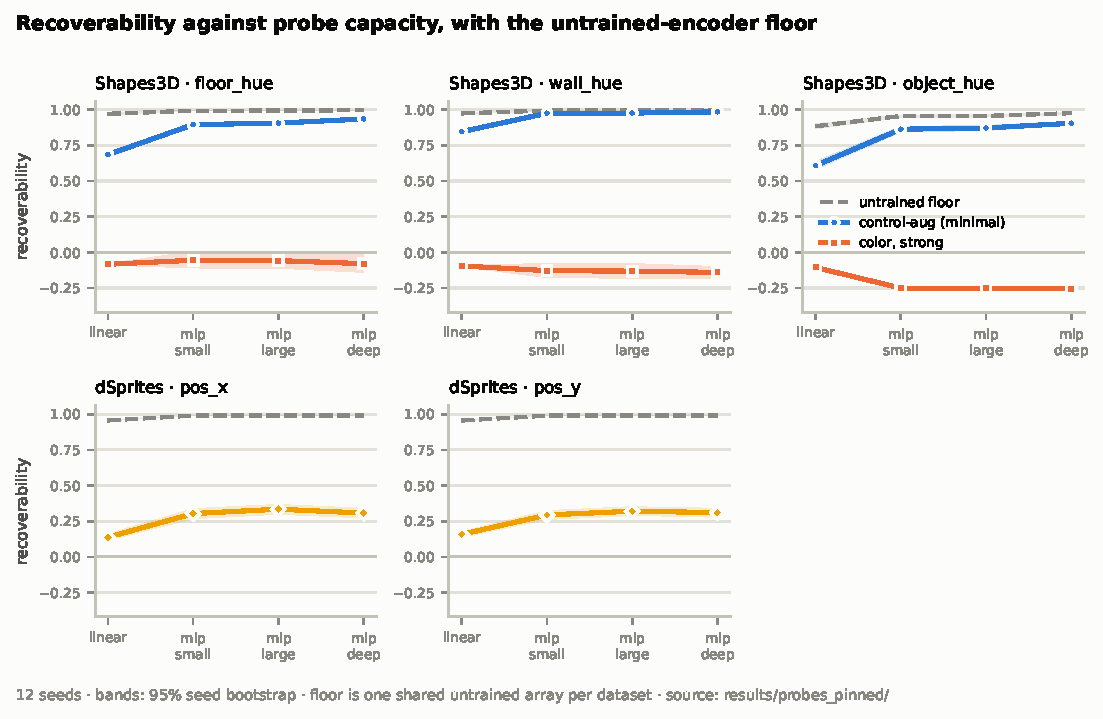
\includegraphics[width=0.86\linewidth]{figures/ladder_floors.pdf}
\caption{Recoverability across probe capacity with the matched untrained-encoder floor. Bands are
95\% seed-bootstrap intervals over twelve seeds, and control and color share one null array. The
Control-aug baseline is exempt from the quality gate under amendment A2.}
\label{fig:ladder}
\end{figure}

The capacity gap inverts the direction the hypothesis predicted. Section~\ref{sec:ladder} quantifies
the upper bias in each gap, which runs in the confirming direction.
On the Control-aug arm five of six readouts are positive with intervals
excluding zero, from wall hue at $+0.115$ $[+0.101, +0.132]$ to floor hue at $+0.224$ $[+0.209,
+0.241]$. On the position arm both targeted readouts are positive too, at $+0.134$ $[+0.116,
+0.151]$ and $+0.117$ $[+0.101, +0.135]$. In the color arm, all three
hue readouts are negative: object hue $-0.241$ $[-0.258, -0.227]$, wall hue $-0.068$ $[-0.102,
-0.034]$, and floor hue $-0.021$ with an interval $[-0.079, +0.044]$ containing zero. Differencing
that gap between the Control-aug and color arms, where the shared floor cancels exactly, gives
$+0.246$ $[+0.170, +0.314]$ on floor hue, $+0.184$ $[+0.147, +0.221]$ on wall hue and $+0.446$
$[+0.429, +0.461]$ on object hue.

\subsection{The closure-fraction dissociation}
\label{sec:kappa}
The closure fraction separates two regimes that receive the same linear-probe classification.
Across fitted probe families the deficit closes in one arm and widens in the other
(Figure~\ref{fig:kappa}).

On floor hue, wall hue and object hue Control-aug returns $\kappa = +0.784$ $[+0.762, +0.808]$,
$+0.900$ $[+0.890, +0.910]$ and $+0.742$ $[+0.718, +0.771]$. The color arm returns $-0.020$
$[-0.075, +0.041]$, $-0.064$ $[-0.096, -0.031]$ and $-0.244$ $[-0.266, -0.225]$. On wall hue and
object hue the intervals are disjoint and have opposite signs. For floor hue, the control interval
is positive while the color interval includes zero.

The linear rung separates these arms and its verdict does not. Linear recoverability there is
$0.6848$, $0.8458$ and $0.6082$ in Control-aug against $-0.0835$, $-0.0952$ and $-0.1056$ in color,
a gap of $0.714$ to $0.941$ of the normalized scale. Yet all six readouts are $\epsilon$-invariant
and null-saturated at that rung, because each trained score sits at or below its own untrained
floor. Thresholding against that floor discards the separation, and only the capacity sweep
recovers the opposing trajectories.

These two arms differ in augmentation composition and gate status. Color applies a photometric
transform alone, Control-aug a crop alone (Table~\ref{tab:conditions}), and Control-aug is the
exempt baseline that fails the quality gate on all twelve seeds (Section~\ref{sec:controls}). They
share the dataset, probe ladder, probe-training size, seed values and untrained-encoder array.

\begin{figure}[tb]
\centering
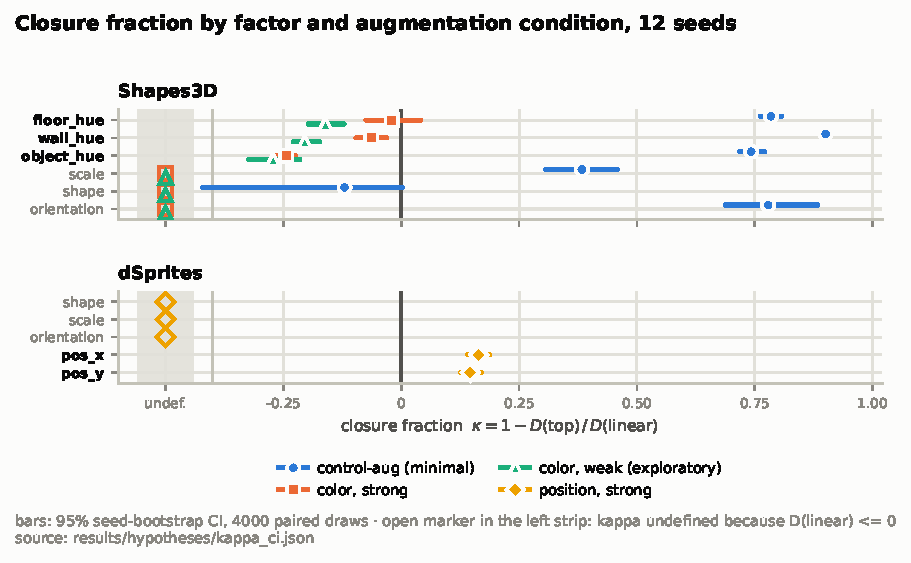
\includegraphics[width=0.88\linewidth]{figures/kappa_dissociation.pdf}
\caption{Closure fraction per factor per condition, twelve seeds, with 95\% seed-bootstrap
intervals from 4{,}000 paired draws. On the three Shapes3D hue factors Control-aug and the color arm
have non-overlapping intervals and point estimates of opposite sign, and one color-arm interval
includes zero. Open markers indicate a nonpositive linear-rung deficit, where $\kappa$ is undefined.
The weak-color arm is exploratory, and Control-aug is exempt from the quality gate under amendment
A2.}
\label{fig:kappa}
\end{figure}

In Control-aug, between three quarters and nine tenths of the linear deficit closes across fitted
probe families, consistent with the linearly inaccessible regime studied by \citet{belrose2023leace}
and \citet{elazar2021amnesic}, while in the color arm the deficit widens.
Section~\ref{sec:disp-results} determines whether that suppression carries displacement below the
calibrated band.

Two floor-free quantities show the same separation. Differencing the capacity gap between arms, as
Section~\ref{sec:gap} does, cancels the shared floor. Absolute control-task performance separates
the two
arms even more sharply. At the
deepest rung a probe recovers the \emph{scrambled} hue map from held-out images at
$\R^{\mathrm{perm}} = 0.817$, $0.982$ and $0.847$ in Control-aug, and at $-0.230$, $-0.217$ and
$-0.278$ in the color arm. Because that scrambled map is a function of the image and has no
ordinal structure, recovering it requires only that the encoder separate the ten hue values.
Control-aug separates them. Color-arm performance remains below the random baseline at every rung,
while the matched untrained encoder reaches at least $0.976$. Thus, the capacity gap, closure
fraction, and control task agree on the direction of the hue separation.

\subsubsection*{Additional closure-fraction results}
Both underlying deficits show the separation before their ratio is taken
(Figure~\ref{fig:plane}). For floor, wall and object
hue, Control-aug falls from $0.286$, $0.128$ and $0.276$ at the linear rung to $0.062$, $0.013$ and
$0.071$ at the top, while the color-arm deficits rise from $1.054$, $1.069$ and $0.989$ to $1.076$,
$1.138$ and $1.230$. Retaining negative $R^2$ allows deficits beyond the normalized unit scale,
as the color arm shows.

Our confirmatory comparison changes both crop and photometric augmentation. A crop is color-blind
while color jitter directly changes hue, and this design does not estimate their separate effects.
Three observations narrow the alternatives. Untargeted geometric factors in the color arm remain
between $0.999$ and $1.000$ and move under the counterfactual certificate. The crop-free weak-color
arm also widens, at object-hue $\kappa=-0.272$ $[-0.323,-0.215]$, which differs from strong color by
$-0.028$ $[-0.085,+0.032]$ and is a non-detection at twelve seeds. An exploratory one-seed
crop-plus-color arm retains hue under the certificate, and its closure fractions fall $34.6\%$ to
$53.5\%$ of the way from Control-aug toward color (Section~\ref{sec:limitations}). We therefore
state the confirmatory result as a difference between augmentation regimes.

Position shows partial closure, at $\kappa=+0.164$ $[+0.141,+0.187]$ for $x$ and $+0.147$
$[+0.126,+0.170]$ for $y$. Five of sixteen confirmatory readouts have nonpositive linear deficits,
so $\kappa$ is undefined on them: scale, shape and orientation in color, and shape and scale in
position. That is also true of the diagnostic dSprites orientation readout.

\subsubsection*{Control-task checks}
Nonlinear probes can trade selectivity for accuracy \citep{belinkov2022probing}, and two
random-label controls check for that. Selectivity at the deepest rung is positive on all six hue
readouts. Control-aug wall hue has the largest closure fraction we measure, $+0.900$, and the
smallest selectivity of the six: a probe on the scrambled map reaches $0.982$ where the true map
reaches $0.985$. That readout therefore supports separation of wall-hue values and says little about
whether their order is represented, which is one reason we report closure fractions per factor.

Recomputing $\kappa$ with both roles on permuted labels preserves the between-arm separation in sign
and approximate magnitude on the three hue factors. For hue, $\kappa$ therefore measures closure of
a value-separability deficit independent of the assigned label order, and ordered and metric
structure stay outside that scope. Appendix~\ref{app:selectivity} gives every per-readout
value with its interval, and reports the two factors on which the two quantities take opposite
signs.

\subsection{Rank-conditional counterfactual displacement}
\label{sec:disp-results}
The widening color-arm deficit is compatible with either retained nonlinear information or
displacement below the measurement resolution. Counterfactual displacement separates these cases
using the calibrated threshold $m^{*}=0.2888$ and the unadjudicated band $[0.0799,1.0445]$.

\begin{figure}[tb]
\centering
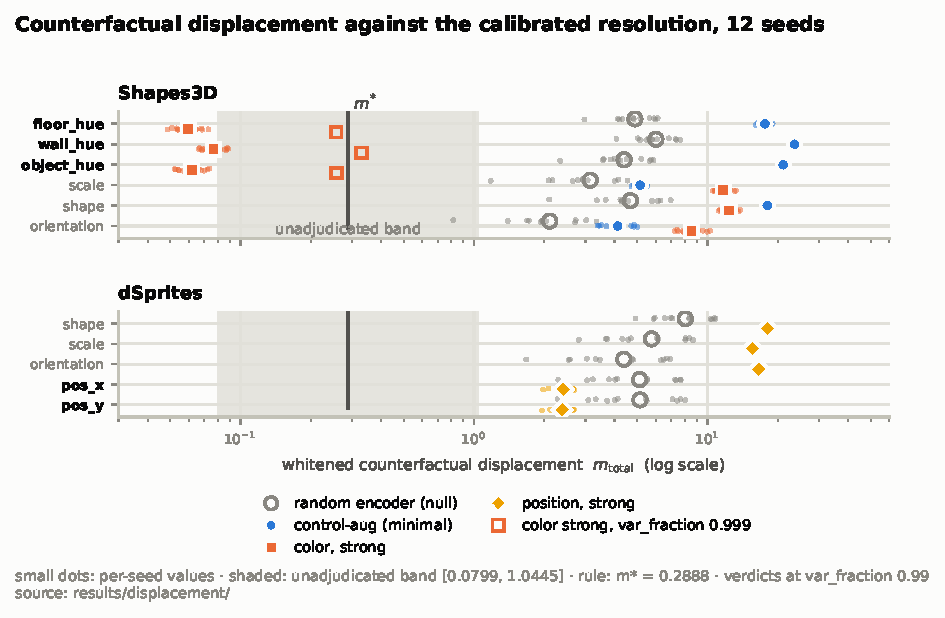
\includegraphics[width=0.88\linewidth]{figures/displacement_certificate.pdf}
\caption{Whitened counterfactual displacement $m_{\mathrm{total}}$ on a log axis for twelve seeds.
Small dots are seed values, the vertical rule is $m^{*}$, and the shaded region is unadjudicated.
The three hue factors fall below the band in color and reach $17.6$ to $23.6$ in Control-aug. Open
squares show color at variance fraction $0.999$.}
\label{fig:disp}
\end{figure}

The same hue factors occupy different regimes across arms (Figure~\ref{fig:disp}). In color, they
measure $m_{\mathrm{total}} = 0.0597$, $0.0766$, and $0.0617$, all below the band. In Control-aug the \emph{same three factors on the same dataset} measured $17.63$, $23.61$ and $21.10$,
all far above it, and the random-encoder null measured $4.89$, $6.01$ and $4.40$. Control-to-color ratios are $295$, $308$ and $342$, a separation spanning between $2.47$ and $2.53$ orders of
magnitude. Non-targeted factors range from $4$ to $24$ in every cell.

The position arm retains both targeted factors at this resolution: $m_{\mathrm{total}}=2.411$ for
$x$ and $2.385$ for $y$, above the band's upper edge of $1.0445$ on all twelve seeds. That reading
transfers the Shapes3D-calibrated $m^{*}$ to dSprites unchanged, where the low-rank fixture makes
\emph{moves} the easier verdict (Appendix~\ref{app:limits}).

Claims of $\epsilon$-destruction below refer only to the color arm, and each is conditional on the
rank the stated variance fraction retains. Floor and object hue are
$\epsilon$-destroyed on all twelve seeds. Wall hue is
$\epsilon$-destroyed on seven seeds and unadjudicated on five. Our preregistered variance-fraction
sweep bounds this conclusion. All three factors are $\epsilon$-destroyed on all seeds at $0.95$;
the primary $0.99$ results are those above; and all are unadjudicated at $0.999$. None is
classified as moving. Read without that condition the verdict is not defined, so the instrument
supports a resolution-dependent failure to separate hue values and not the literal absence of
information from a deterministic encoder.

\subsubsection*{Rank sensitivity}
The absolute scale varies with the retained whitening rank; every reported rank is a mean over
twelve seeds. At variance fractions $0.95$, $0.99$ and $0.999$, mean color-arm rank is $56$, $106$
and $210$, while floor-hue $m_{\mathrm{total}}$ is $0.0212$, $0.0597$ and $0.2571$. The fitted
exponent in rank is $+1.90$ for floor hue, $+1.89$ for wall hue and $+1.84$ for object hue;
untargeted factors give $+0.54$ to $+0.74$. Our calibrated threshold therefore applies at a stated
retained rank.

Within the color arm the matched trained-to-untrained ratio is the more stable companion. It
spreads $1.5$ to $2.1$ across the sweep while $m_{\mathrm{total}}$ changes by about $12$, and the
trained encoder displaces hue only $1.1\%$ to $2.3\%$ as far as its matched untrained counterpart.
Paired seed bootstraps at the primary fraction put every hue interval below $0.017$, while the same
encoders displace shape, scale and orientation $2.65$ to $4.05$ times as far as that null
(Appendix~\ref{app:sweep}).
That stability belongs to this arm alone, since in the control and position arms the same ratio
varies by as much as a factor of $105$ and crosses parity at $0.999$. We therefore keep the preregistered
$m_{\mathrm{total}}$ verdict as primary and report the ratio as an arm-specific companion.
Appendix~\ref{app:sweep} gives the per-arm spreads, the rank paths, and Figure~\ref{fig:disprank}.

\subsubsection*{Scale qualifications and instrument checks}
Separate whitening gives the trained and untrained roles different ranks, $435.5$ and $56.8$ in
Control-aug. Normalizing each role by its own $m_{\mathrm{ctx}}$ reduces the control-to-color separation from $295$--$342$ to $154$--$182$, still about $2.2$ orders of magnitude
(Appendix~\ref{app:sweep}). The whitening diagnostic $m_{\mathrm{ctx}}/\sqrt{2k}$ ranges from $0.84$ to $1.01$ over every seed, role, factor and cell at the primary fraction, on a
preregistered rule that sets the target at $1$ and leaves the tolerance qualitative. The reduction
controls follow their measured input leak (Appendix~\ref{app:reduction}).

The preregistered correlation between displacement and capacity gap is not evaluable. Exclusions
leave one eligible readout per cell, three in total and all of the same metric type, while the test
requires at least three commensurable readouts per group, and pooling across cells would violate the
stated design.

\subsection{The preregistered verdicts}
\label{sec:prereg}
Section~\ref{sec:design} states the four rules. Each was fixed before analysis.

\textbf{H1 is confirmed} on seven readouts: floor, wall and object hue, scale and orientation in
Control-aug, plus $x$ and $y$ in position. That confirming set is unchanged under the fixed-$0.05$
sensitivity, and confirmations concentrate in Control-aug, which is the inversion documented in
Section~\ref{sec:gap}.

No color-arm readout confirms H1.

\textbf{H2 is confirmed}: twelve of twenty-three within-type pairs survive Holm correction, five
in color, five in Control-aug and two in position. This is within-cell heterogeneity between
targeted and untargeted factors, and eleven remaining comparisons are non-detections at twelve
seeds. Every one of the twelve realized-family survivors also survives A6's maximal-family
sensitivity over all five designed cells, so the H2 verdict holds on the designed family as well
(Appendix~\ref{app:amendments}).

\textbf{H3 is refuted.} Ten readouts remain $\epsilon$-invariant at every rung, but all ten are
null-saturated: three color-arm hue factors, five Control-aug factors and both position factors.
Only Shapes3D shape and dSprites shape retain usable headroom. The frozen one-sided variant confirms
H3 on Control-aug shape, which lies at the untrained floor and is recovered by the two-sided
primary, and both rules agree on every other readout. H3 therefore reflects the benchmark ceiling
documented in Section~\ref{sec:headroom}, which amendment A14 recorded before the blind broke. The
refutation describes our instrument's headroom on these benchmarks and says nothing about
invariance in the representations.

\textbf{H4 is not evaluable.} Its rule requires the encoder-minus-projector gap to widen across two
augmentation strengths, whereas the realized grid has one, so we report the sign component descriptively below.

\textbf{The flip count is 1}, on Control-aug shape, with a seed-bootstrap mean of $0.196$ and a
95\% interval of $[0,1]$. The null-saturation-excluded two-sided count is also $1$. Each frozen
one-sided variant returns $0$ under both the factor-specific and fixed-$0.05$ thresholds, with or
without the saturation exclusion. We report all six variants because the count is unstable and was
defined to include only non-targeted readouts.

\textbf{The encoder--projector sign component}\label{sec:h4} survives Holm correction in fourteen
cell-factor-rung combinations and reverses at the color arm's linear rung. That pattern is
capacity-dependent and descriptive, not an H4 test, because the widening component is unavailable,
and it is why we probe the backbone throughout (Appendix~\ref{app:h4}).

\section{Discussion}
\label{sec:discussion}

\subsection{Interpretation and implications}
The experiments suggest a three-part audit. First, test an untargeted factor before interpreting a
targeted one. One linear probe flagged both
correspondence failures here, and the ladder then separated the closing deficit from the
persistent one. In-plane image rotation and 3D camera azimuth are different group actions, while our
scale condition failed an encoder-quality gate and
two exploratory measurements, one of them a single-seed pilot, point at its single-transform recipe
on a hue-dominated dataset where a color shortcut stays open. In both arms correspondence turned on
a measurement or an
argument beyond the augmentation's name. This gate is strongest on a complete factorial grid, and
natural-image use would require a labeled factor that
the augmentation plausibly preserves.

Second, vary probe capacity when the random-encoder comparison leaves adequate headroom. A linear
probe gives the same hue verdict in the color and Control-aug arms, yet the underlying regimes
differ. In Control-aug, an MLP closes $74\%$ to $90\%$ of the linear deficit, so hue recoverability
ends within $0.013$ to $0.071$ of the untrained floor; in color the deficit widens and even a
permuted value map remains unrecoverable. The first matches the ``present but linearly
inaccessible'' case formalized by \citet{belrose2023leace}, and the second is a broader failure of
value separability at the tested capacities.

Third, use paired counterfactuals when the dataset supplies them. After a conservative rank
normalization, color-arm hue displacement remains twenty to twenty-three times smaller than in
Control-aug, against a raw gap of $2.5$ orders of magnitude. The ladder and permuted-label task are
both probe based and closely related for hue, so counterfactual displacement supplies the independent
check: it fits no predictor and reaches the same separation. Extending this instrument beyond
factorial grids would require paired scenes, a matched untrained null and a calibration fixture;
EditCLEVR is one possible setting \citep{karnam2026editclevr}.

\subsection{Scope of claims and limitations}
\label{sec:limitations}
We confine our claims to recoverability from frozen small SimCLR encoders on Shapes3D and dSprites,
at the stated probe capacities and augmentation settings, over twelve seeds.

\subsubsection*{Global scope}
The study covers one self-supervised objective, one confirmatory strength, $64\times64$ synthetic
images, a small backbone and an NT-Xent batch of 512, so natural images, larger models, other
objectives and other strengths lie outside what these measurements estimate. High
random-encoder floors further limit fitted-probe claims. We accompany each verdict with absolute
levels and a saturation flag, since ``no detectable gain'' leaves open whether a deterministic
encoder kept the information.

Factor identity also varies with dataset. The central color-versus-Control-aug dissociation is a
Shapes3D result on three hue factors, and the dSprites position arm is intermediate on both
instruments, so that contrast is tested on one dataset only and heterogeneity tests are within-cell.
Our four probe families form a practical capacity ladder, and a theory of capacity scaling is a
separate question \citep{lee2026shallow}. Projector comparisons are descriptive, and
non-significant tests are non-detections at twelve seeds after Holm correction.

\subsubsection*{Bearing on the main interpretation}

\textbf{Rank sensitivity.} At variance fraction $0.999$, every color-arm hue verdict becomes
unadjudicated; none becomes moving. The calibration fixture is a rank-1 fully shared ramp, where
$m_{\mathrm{shared}}$ and $m_{\mathrm{total}}$ agree within $10^{-4}$. Color-arm hue fields have
effective rank $45.6$--$47.0$ and shared fractions $0.097$--$0.218$, so their context-dependent
movement grows as more directions are retained. A post-hoc score using $m_{\mathrm{shared}}$ gives
$\epsilon$-destruction on all seeds at $0.95$ and $0.99$, and on eleven or twelve seeds at $0.999$;
we report it as robustness evidence, since the preregistered scale is $m_{\mathrm{total}}$.

Applying the color arm's own fitted rank exponent reduces the raw $295$-fold floor-hue contrast to
about $20$, and conservative corrections leave a $20$--$23$ separation across all three hues.
Because the fixture has lower rank than the measured fields, its threshold makes movement easier to
declare. The observed $\epsilon$-destruction is conservative in that direction. Raw magnitudes and
trained-to-null ratios are not commensurable across arms with dissimilar ranks, so primary verdicts
compare each arm with its matched null at its own rank (Appendix~\ref{app:sweep}).

\textbf{Augmentation confounding.} The color and Control-aug cells share no transform: adding color
jitter also removes a crop (Table~\ref{tab:conditions}), so the two effects remain confounded in
this design. The three observations in Section~\ref{sec:kappa} narrow the alternatives, and the cell
that would settle them carries both transforms. Here that cell exists only as a one-seed pilot,
which also differs in crop scale, horizontal flip, photometric strength and training length
(Appendix~\ref{app:exploratory}). It associates cropping with whether hue survives, and color jitter
with how much of the linear deficit closes. Separating the two causal effects needs the same cell at
twelve seeds, which is the augmentation follow-up this calls for.

\textbf{Control quality.} Control-aug clears its quality gate on zero of twelve seeds and remains
under a preregistered design-role exemption. It is weaker than color on shape and scale
($0.737$, $0.321$ versus $1.000$, $0.999$), so overall encoder quality could contribute to the
regime difference. Yet both arms reach similar NT-Xent loss ($4.949$ versus $4.953$), uniformity
($-3.883$ versus $-3.822$) and median alignment ($1.0\times10^{-4}$ versus $6.9\times10^{-5}$, with two
color seeds at $2.5\times10^{-3}$ and $4.2\times10^{-3}$, Appendix~\ref{app:training}). Color-arm
suppression is also selective within each encoder: shape, scale and orientation score
at least $0.999$ and displace $2.65$ to $4.05$ times as far as their matched untrained null, where
hue displaces $0.012$ to $0.014$ times as far (Appendix~\ref{app:sweep}). Hue is
$\epsilon$-destroyed at fractions up
to $0.99$, on all twelve seeds for floor and object hue and on seven for wall hue. A replicated
crop-bearing color arm that passes the gate would address this concern as well.

\subsubsection*{Bearing on the mechanism}

The preregistered mechanism test is not evaluable, for the reason
Section~\ref{sec:disp-results} gives, and we kept that rule fixed after unblinding. A benchmark with
more non-saturated, within-type factors is needed to test whether displacement predicts the capacity
gap.

Whitening is exactly stable under orthogonal maps and approximately stable under general invertible
ones, and we tested that for displacement alone. The closure fraction's coordinate stability remains
open (Appendix~\ref{app:limits}).

\subsubsection*{Bearing on the two excluded arms}
We excluded scale on the shape gate before targeted-factor analysis, and a one-seed recipe control
then restored shape to a perfect score under the identical affine zoom, which implicates the
single-transform recipe at that seed. We excluded rotation analytically.

\subsubsection*{Affecting precision}

Optimization leaves an upper bias in each capacity gap, quantified in
Section~\ref{sec:ladder}, and capacity and optimization remain partly coupled. A compositional-split
control overturned an interim attribution of the high untrained floor to random-index splitting: the
floor persists and belongs to the factor and untrained architecture. Random-label controls, fixed
probe-train size and test-only reporting limit probe overfitting without eliminating it
\citep{belinkov2022probing}. With twelve seeds, small effects may escape the Holm-corrected Wilcoxon
test, so null results remain non-detections. Appendix~\ref{app:limits} adds one boundary seed at
variance fraction $0.95$ and the monotonicity diagnostic we exclude from verdicts.

\section{Conclusion}
\label{sec:conclusion}

Invariance claims depend on the instrument used to measure them. Our preserved-factor audit removed two of five designed
conditions before targeted-factor analysis, one on the shape gate and one on a group-action
argument. A four-rung probe ladder
then separated two cases that a linear-probe invariance verdict classifies identically: the deficit
closes across fitted probe families in Control-aug and widens in color, across two arms that apply
disjoint augmentation sets and differ in gate status. Counterfactual displacement, which fits no probe, independently places color-arm floor
and object hue below the calibrated resolution on all twelve seeds, and wall hue on seven of them,
at variance fractions at or below $0.99$. All three become unadjudicated at $0.999$.

The practical audit is modest: check an untargeted factor, compare several probe
capacities with a matched untrained encoder, and use paired displacement when exact counterfactuals
exist. Its limits matter as much. Random-encoder floors leave little fitted-probe headroom,
displacement is rank-sensitive, and the study covers small SimCLR models on synthetic grids. A larger factorial
benchmark with more non-saturated factors would permit the preregistered mechanism test and provide
the most informative replication.


\subsubsection*{Reproducibility Statement} One command regenerates every number and
figure from the released probe stacks and displacement records, and reproducing those artifacts from
scratch requires retraining from the released configurations because checkpoints are not
distributed. \texttt{make trace} checks 923 assertions from a curated list and \texttt{make
manifest-check} verifies released artifacts against recorded SHA-256 values, both from a clean
export of the repository. The manifest records two withheld classes: large checkpoints, and hand-set
decision-rule test tables whose values could be mistaken for measurements. Both datasets are public,
and Appendix~\ref{app:artifacts} describes the repository, which holds the code, frozen
preregistration and fifteen amendments.


\bibliography{references}
\bibliographystyle{tmlr}

\appendix
\section{Notation and interpretation limits}
\label{app:notation}
Table~\ref{tab:notation} collects every symbol used in the paper, with the condition that makes each
quantity undefined or uninformative.

\begin{table}[tb]
\centering
\caption{Notation and conditions that limit interpretation.}
\label{tab:notation}
\small
\begin{tabular}{l l l}
\toprule
Symbol & Quantity & Undefined or uninformative when \\
\midrule
$\R(F,c)$ & recoverability of factor $F$ at capacity $c$ (Eq.~\ref{eq:RS}) & --- \\
$\R^{\mathrm{perm}}$ & recoverability of the permuted label map & --- \\
$\Sel(F,c)$ & selectivity, $\R - \R^{\mathrm{perm}}$ (Eq.~\ref{eq:RS}) & $F$ categorical ($\Sel \equiv 0$) \\
$\G(F,c)$ & encoder gain over the untrained null (Eq.~\ref{eq:G}) & $\R^{\mathrm{random}}$ reaches $0.90$ \\
$\tilde{\G}$ & headroom-normalized gain, $\G/(1-\R^{\mathrm{random}})$ & denominator near zero \\
$\Delta_{\G}(F)$ & capacity gap, $\G(F,c_4) - \G(F,c_1)$ (Eq.~\ref{eq:G}) & --- \\
$D(F,c)$ & deficit, $-\G(F,c)$ & --- \\
$\epsG$, $\epsilon_D$ & detection thresholds from the random-versus-random null & --- \\
$\kappa(F)$ & closure fraction (Eq.~\ref{eq:kappa}) & $D(F,c_1) \le 0$ \\
$m_{\mathrm{total}}$ & mean whitened counterfactual displacement (Eq.~\ref{eq:mtotal}) & compared across unlike rank \\
$m_{\mathrm{shared}}$ & norm of the context-averaged displacement (Eq.~\ref{eq:mtotal}) & --- \\
$m_{\mathrm{ctx}}$ & displacement between contexts at fixed $F$ & --- \\
$m^{*}$ & calibrated resolution, $0.2888$ (Eq.~\ref{eq:mstar}) & inside the band $[0.0799, 1.0445]$ \\
$k$ & retained whitening rank at the stated variance fraction & --- \\
\bottomrule
\end{tabular}
\end{table}

\section{Training diagnostics}
\label{app:training}
Table~\ref{tab:training} reports optimization diagnostics by arm. Color and Control-aug have
similar final NT-Xent and uniformity, and their alignment values overlap on ten of the twelve
color-arm seeds; the remaining two, at $2.5\times10^{-3}$ and $4.2\times10^{-3}$, are far above
the color arm's own median of $6.9\times10^{-5}$, the comparison Section~\ref{sec:limitations} uses
when it assesses encoder quality. Position-arm alignment runs from $2.6\times10^{-3}$ to
$1.1\times10^{-2}$ with uniformity above $-3.88$, and our crop-plus-color pilot has the study's
highest NT-Xent at $4.9875$, so these two arms are unsuitable for matched-optimization
comparisons with the central pair.

\begin{table}[t]
\centering
\caption{Training diagnostics by arm. Ranges give the minimum and maximum across seeds. The color
and Control-aug arms have comparable NT-Xent and uniformity; the other arms are reported
descriptively (Section~\ref{sec:limitations}).}
\label{tab:training}
\small
\begin{tabular}{l c c c c c}
\toprule
Arm & Seeds & Epochs & Final NT-Xent & Alignment & Uniformity \\
\midrule
Color, strong & 12 & 50 & 4.9527--4.9529 & $5.5\times10^{-5}$--$4.2\times10^{-3}$ & $-3.834$--$-3.815$ \\
Control-aug & 12 & 50 & 4.9488--4.9490 & $9.3\times10^{-5}$--$1.2\times10^{-4}$ & $-3.885$--$-3.880$ \\
Position \textsuperscript{$\dagger$} & 12 & 50 & 4.9638--4.9652 & $2.6\times10^{-3}$--$1.1\times10^{-2}$ & $-3.761$--$-3.728$ \\
Color, weak \textsuperscript{e} & 12 & 50 & 4.9490--4.9492 & $4.8\times10^{-5}$--$7.7\times10^{-5}$ & $-3.884$--$-3.879$ \\
Crop+color \textsuperscript{e} & 1 & 100 & 4.9875 & $1.1\times10^{-2}$ & $-3.691$ \\
\bottomrule
\end{tabular}
\\[2pt]
{\footnotesize \textsuperscript{e} exploratory, in no confirmatory family.
\textsuperscript{$\dagger$} One position-arm seed has no metrics summary. Its final training-log
row records the same three quantities, as it does for every seed that has both, and all three of its
values fall inside the printed ranges.}
\end{table}

\section{Reduction controls and their measured leak}
\label{app:reduction}
Two input-side reductions accompany Section~\ref{sec:certificate}: luminance
grayscale and the value channel $\max(R,G,B)$. Neither is ground truth, and the reason is measured.
On raw Shapes3D images with no encoder involved, we swept object hue over all
ten values at a fixed context. Luminance grayscale leaves a mean per-pixel range across hue of
$16.62/255$, with $15.5\%$ of pixels moving above $1/255$ and a minimum pairwise $L_2$ between hue
values of $61.4$: hue at fixed saturation and value maps to different luminances, so grayscaling
\emph{reduces} hue without removing it and a CNN recovers the ten values from what remains. The
value channel is hue-invariant at fixed saturation and value by construction and measures about
sixteen times tighter ($1.06/255$, $5.9\%$ of pixels, minimum pairwise $L_2$ of $2.0$). Shading,
specular highlights and compression break that assumption, so no
transform of the released images is a provable zero.

Measured behavior matches. Under grayscale the three hue factors give $m_{\mathrm{total}}$ values
of $1.11$, $1.48$ and $1.02$; under the value channel they give $0.90$, $1.38$ and $1.07$. Neither
collapses hue displacement to zero, exactly as the leak measurement predicts. Both are therefore
strong-reduction controls with their leak stated: an instrument that failed to fire under them would
be broken, and firing under them is necessary and not sufficient. Neither enters a confirmatory
family, and the threshold-setting device is instead the synthetic fixture of
Equation~\ref{eq:mstar}, where the answer is known exactly.


\section{Encoder versus projector, in full}
\label{app:h4}
The sign component of H4 is significant after Holm on fourteen cell-factor-rung combinations: floor
hue and wall hue in the color arm at the three MLP rungs, and $x$ and $y$ position in the position
arm at all four rungs. Those differences are of the size the test of \citet{cosentino2022geometry}
would predict, for instance $+0.149$ $[+0.094, +0.207]$ for color-arm floor hue at the small MLP
rung, and at the linear rung in the color arm the sign reverses, at $-0.109$ $[-0.128, -0.090]$ for
the same readout. Because the widening component cannot be evaluated at a single strength, none of
this is a test outcome. It is a descriptive observation that the encoder-versus-projector
distinction is visible here and is capacity-dependent, and it is why we probe the
backbone throughout.

\section{Selectivity and the control-task closure fraction}
\label{app:selectivity}
This appendix holds the per-readout evidence behind the two control-task results of
Section~\ref{sec:kappa}.

\subsection*{Selectivity by readout}
We use the random-label control to check the accuracy-for-selectivity trade in Control-aug, where
recoverability approaches $0.9$.

\begin{figure}[tb]
\centering
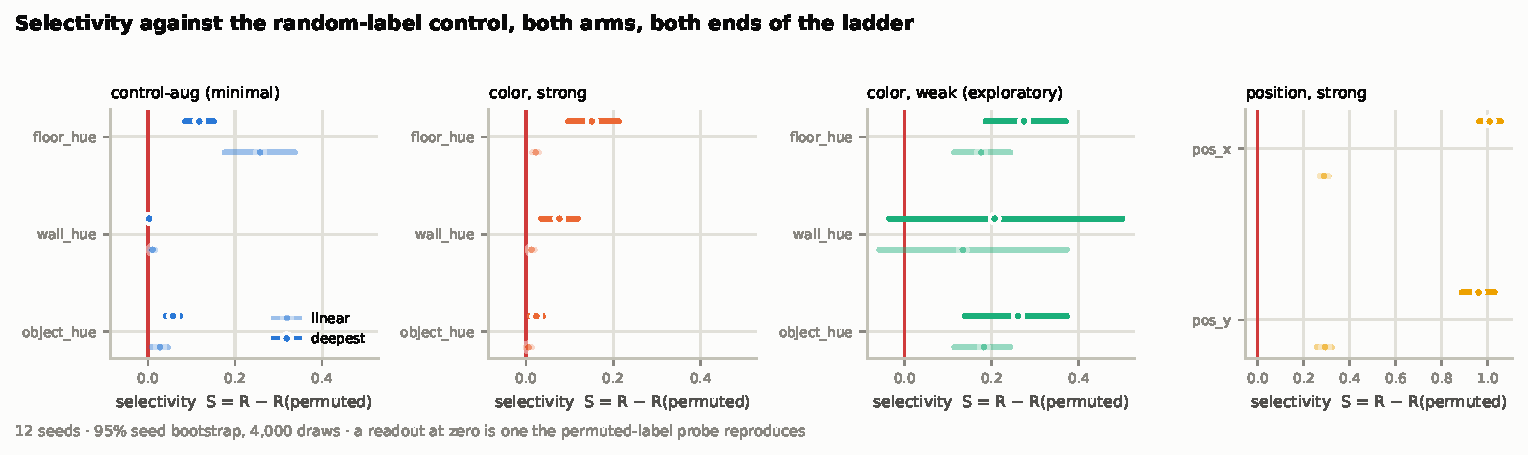
\includegraphics[width=\linewidth]{figures/selectivity.pdf}
\caption{Selectivity $\Sel = \R - \R^{\mathrm{perm}}$ at the linear and deepest rungs, for every arm
and both ends of the ladder, with 95\% seed-bootstrap intervals. The three Shapes3D panels share an
axis. The control task permutes each factor's value-to-target map identically across splits, so the
permuted label stays a function of the image and is recoverable exactly to the extent that the
encoder separates that factor's values.}
\label{fig:sel}
\end{figure}

Pairing trained and untrained encoders controls architecture and data splits, but it does not cancel
probe memorization because the roles occupy different performance regimes. Untrained encoders score from $0.88$ to $0.997$ on these factors, whereas the trained color arm
remains below zero at every rung. We therefore rely on the random-label task for this check.

Figure~\ref{fig:sel} reports selectivity by readout. At the deepest rung the color
arm gives $+0.151$ $[+0.096, +0.215]$, $+0.076$ $[+0.034, +0.118]$ and $+0.023$ $[+0.009, +0.038]$,
and Control-aug gives $+0.118$ $[+0.086, +0.150]$ on floor hue, $+0.058$ $[+0.041, +0.074]$ on
object hue and $+0.003$ $[+0.002, +0.004]$ on wall hue. Wall hue carries this paper's largest
$\kappa$ at $+0.900$ and a top-rung selectivity of three thousandths: a probe on the scrambled map
reaches $0.982$ where the true map reaches $0.985$. That interval excludes zero, but the effect is
negligible beside the absolute level, which is why we report closure fractions per factor rather
than averaged across hues.

\subsection*{The control-task closure fraction in full}
We recomputed $\kappa$ with both roles evaluated on permuted labels, using twelve random encoders,
probe-train size $2{,}000$, $1{,}000$ steps and $4{,}000$ paired
bootstrap draws. Its recomputed random linear rung differs from the shipped stack by
$3.31\times10^{-5}$, below the $5\times10^{-3}$ equivalence threshold, and all nine defined values
of $\kappa$ agree within $0.004$.

Write $\kappa^{\mathrm{perm}}$ for this control-task closure fraction. On the three hues it is
$+0.641$, $+0.892$ and $+0.573$ in Control-aug,
against the recomputed run's own $\kappa$ of $+0.785$, $+0.900$ and $+0.739$, and $-0.198$, $-0.145$
and $-0.365$ in the color arm against that run's $-0.020$, $-0.064$ and $-0.244$;
Table~\ref{tab:kappanull} gives every interval and all defined pairs. For wall
hue the control-task value reproduces $99.1\%$ of the paper's largest closure fraction.
On color-arm floor hue, its magnitude is $9.8$ times the observed point estimate. So
$\kappa^{\mathrm{perm}}$ preserves the between-arm separation in sign and approximate magnitude for
the hue factors, which shows that $\kappa$ does not isolate ordered label structure in these cells.

\begin{table}[t]
\centering
\caption{Observed and control-task closure fractions for the nine defined Shapes3D readouts. Both
roles use permuted labels for $\kappa^{\mathrm{perm}}$. Values come from twelve random and
twenty-four
trained encoders with $4{,}000$ paired bootstrap draws. The $\kappa$ column is this run's own
recomputation, which agrees with Section~\ref{sec:kappa} within $0.004$. The dSprites control was
not run.}
\label{tab:kappanull}
\small
\begin{tabular}{l l cc cc}
\toprule
Arm & Factor & $\kappa$ & 95\% CI & $\kappa^{\mathrm{perm}}$ & 95\% CI \\
\midrule
Color, strong & Floor hue & $-0.020$ & $[-0.075, +0.041]$ & $-0.198$ & $[-0.257, -0.129]$ \\
               & Wall hue & $-0.064$ & $[-0.097, -0.030]$ & $-0.145$ & $[-0.184, -0.107]$ \\
               & Object hue & $-0.244$ & $[-0.267, -0.225]$ & $-0.365$ & $[-0.432, -0.302]$ \\
\midrule
Control-aug & Floor hue & $+0.785$ & $[+0.760, +0.809]$ & $+0.641$ & $[+0.598, +0.680]$ \\
            & Wall hue & $+0.900$ & $[+0.890, +0.910]$ & $+0.892$ & $[+0.869, +0.909]$ \\
            & Object hue & $+0.739$ & $[+0.713, +0.767]$ & $+0.573$ & $[+0.438, +0.669]$ \\
            & Scale & $+0.383$ & $[+0.306, +0.459]$ & $-0.205$ & $[-0.347, -0.055]$ \\
            & Shape & $-0.120$ & $[-0.410, -0.015]$ & $-0.142$ & $[-0.421, -0.042]$ \\
            & Orientation & $+0.779$ & $[+0.694, +0.885]$ & $-0.405$ & $[-0.493, -0.281]$ \\
\bottomrule
\end{tabular}
\end{table}

Because the permuted map is fixed across splits, recovery requires only that the encoder separate
the factor's values, which is what distinguishes a control representation from a color-arm
representation here. Ordered and metric structure remain outside the scope of this control.

For other factors the real and permuted tasks differ more. On the untrained linear rung, permutation
reduces recoverability by $+0.024$ on wall hue, $+0.057$ on floor hue, and $+0.110$ on object hue,
compared with $+0.665$ on scale, $+0.529$ on orientation, and $-0.0002$ on categorical shape. For
scale, $\kappa=+0.383$ $[+0.306,+0.459]$ while $\kappa^{\mathrm{perm}}=-0.205$
$[-0.347,-0.055]$; for orientation the corresponding values are $+0.779$
$[+0.694,+0.885]$ and $-0.405$ $[-0.493,-0.281]$. Those opposite signs confirm that the control-task
quantity diverges from $\kappa$ when permutation changes the prediction problem substantially.

\subsection*{The deficit plane}

\begin{figure}[tb]
\centering
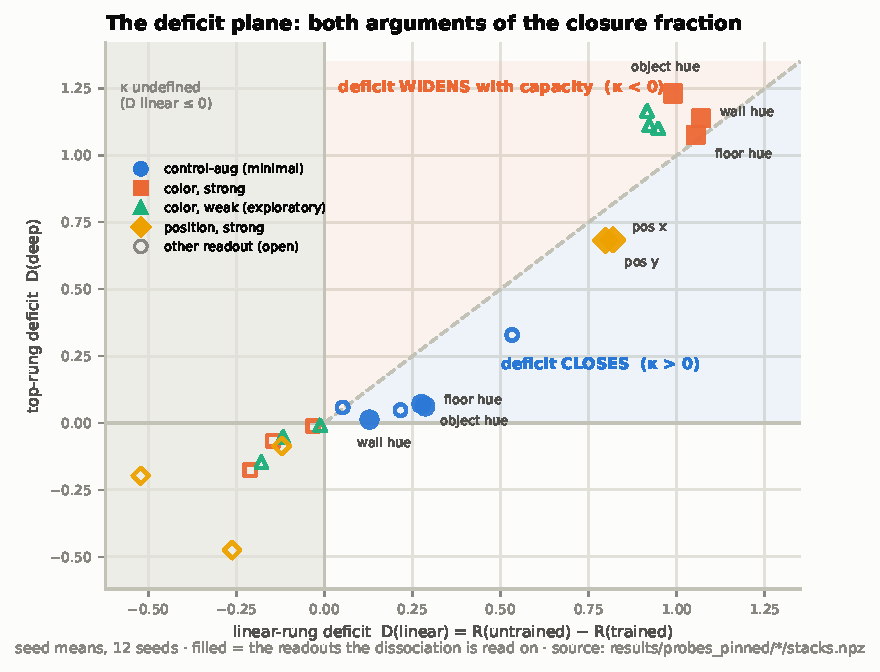
\includegraphics[width=0.62\linewidth]{figures/deficit_plane.pdf}
\caption{The deficit plane, which shows both arguments of the closure fraction. Each marker is
one readout at its linear-rung and top-rung deficit, seed means over twelve seeds. The diagonal
is $\kappa = 0$ and the horizontal axis is $\kappa = 1$, so closure is the region below the
diagonal and widening the region above it. Values left of the vertical axis have a nonpositive
linear deficit, where $\kappa$ is undefined. Filled markers identify the hue comparison.
Separation is visible in both deficits as well as their quotient. The Control-aug points use the
A2 baseline exemption.}
\label{fig:plane}
\end{figure}

\section{Probe-build details}
\label{app:probebuild}
Every rung uses the same probe build. We standardize inputs per dimension on probe-train statistics
and do the same for continuous targets, which matters because $R^2$ is invariant
under an affine map applied to both target and prediction, while an unstandardized target forces the
probe to reach a large mean through a weight-decayed output bias. Our step budget cannot do that,
and the cost falls hardest on the linear rung. We train with Adam at learning rate $10^{-3}$ and
batch size 4{,}096, and choose weight decay from $\{0, 10^{-4}, 10^{-3}, 10^{-2}\}$ on the
validation split and never on test, so the tuning \emph{budget} is rung-uniform by construction. The
selected \emph{value} need not be. The selected values are unavailable in the
released artifacts and would require retraining to recover, so we cannot report whether the penalty
was constant across rungs; Section~\ref{sec:ladder} states what follows for monotonicity.
Biases are exempt from weight decay, since decaying the output bias
penalizes the probe for representing the target mean and does so unevenly across rungs. We report on
the probe-test split only.

\textbf{The rungs nest as function classes.} Since $\mathrm{ReLU}(a) - \mathrm{ReLU}(-a) = a$, a
rung represents its predecessor exactly whenever twice the output dimension is at most the next
hidden width. That holds at every step here, with output dimension at most four against widths 64,
256 and 128, so parameter count orders a real inclusion chain of hypothesis classes.

\textbf{Realized monotonicity of the ladder.} Across the three confirmatory cells, with the shared
untrained array counted once per dataset, $114$ of the $207$ declining rung-to-rung steps exceed the
linear-rung optimizer budget, and the trained role alone contributes $143$ of $612$ declines. We
estimate that budget from two implementations of the linear probe on
the random encoder's shape readout, which return $0.9082$ from a convex solver and $0.8290$ from the
ladder's Adam probe.

\textbf{The linear rung in the denominator of $\kappa$.} Because calibration measures the
random-encoder role alone, the net sign of its effect on $D(F,c_1)$ is unknown. We therefore
recompute $\kappa$ at $D(F, c_1) \pm$ the arm's own budget. On thirteen of the fourteen readouts
where $\kappa$ is defined, the exploratory weak-color arm's three hues among them and eleven
confirmatory, this moves it by at most $0.014$ and the dissociation is untouched: Control-aug wall
hue runs $+0.892$ to $+0.908$ against a point estimate of $+0.900$, and the color arm's hue
readouts move by at most $0.013$. Control-aug shape is less stable. Its linear-rung deficit is
$0.0520$, so the budget is $19\%$ of the denominator and $\kappa$ spans $-0.385$ to $+0.059$ under
it. We report that readout as unresolvable on this instrument. Its point estimate is $-0.120$.

\textbf{A bias-corrected interval for $\kappa$.} As a ratio estimator, $\kappa$ is especially
sensitive to its denominator. A
bias-corrected and accelerated recomputation changes each endpoint by at most $0.0195$ and widens no
interval by more than a factor of $1.062$. Control-aug shape is the exception in interpretation: its
upper endpoint changes from $+0.0022$ to $-2\times10^{-5}$, while an independent recomputation gives
$[-0.410,-0.015]$ (Table~\ref{tab:kappanull}), so we classify that readout as unresolvable and keep
the preregistered percentile interval as primary.

\textbf{Two renormalizations we examined and set aside.} We asked whether
$\kappa$ could be made headroom-normalized by dividing each rung's deficit by that rung's own
untrained floor. It cannot, for two reasons. The result is a deterministic reparameterization,
$\tilde{\kappa} - \kappa = (1 - \kappa)\bigl(1 - \R^{\mathrm{random}}(F, c_1) /
\R^{\mathrm{random}}(F, c_4)\bigr)$, whose floor ratio runs $0.906$ to $0.979$ here; it moves no
verdict, and on the Control-aug hue readouts it cannot move $\kappa$ by more than $0.025$, so
it does not test the concern it appears to answer.
It also presumes the deficit is bounded by the floor it divides by, which is false on the readouts
the result rests on: the color arm's linear-rung deficits run $0.99$ to $1.07$ against floors of
$0.88$ to $0.97$. The preregistered $\tilde{\G}$ scale, dividing by $1 -
\R^{\mathrm{random}}$, is not usable either: at the top rung that denominator is $0.0027$ to
$0.0243$ on the Control-aug hue readouts with a seed coefficient of variation of $0.30$ to $0.42$,
the estimability problem the null-saturation gate exists to flag. We rest the dissociation on the
floor-free evidence of Section~\ref{sec:closuredef} instead.

\section{Released artifacts and regeneration}
\label{app:artifacts}
The repository contains the training, probing, displacement and figure code, and the run
configurations for every condition, including the two excluded and the three exploratory ones, the
recipe pilot's among them as \texttt{configs/run/scale\_recipe\_control.yaml}. One of those
configurations, the crop-plus-color arm's, we reconstructed from that run's logs, and its header
says
so. The repository also holds the per-cell recoverability stacks, the displacement records at all
three variance fractions, and a CSV table beside every figure carrying its plotted values. Encoder
training used a single consumer GPU at roughly one hour per encoder seed, and the closure-fraction
bootstrap, the hypothesis layer, the certificate's verdict step and the figures run on a laptop from
the released stacks.

The closure fraction's control-task null of Section~\ref{sec:kappa} and the variance-fraction sweep
of Section~\ref{sec:disp-results} on the control and position arms both ship as the notebook that
ran them, which states before it runs which sentence of this paper each possible outcome changes. In
both cases the outcome weakened a sentence in an earlier draft.

\section{Rank sensitivity of the displacement scale}
\label{app:sweep}
\subsection*{Color-arm ratios across the sweep}
The matched trained-to-untrained ratio summarized in Section~\ref{sec:disp-results} runs
$(0.0113, 0.0122, 0.0218)$ on floor hue, $(0.0108, 0.0127, 0.0229)$ on wall hue and
$(0.0194, 0.0140, 0.0210)$ on object hue, each across variance fractions $0.95$, $0.99$ and
$0.999$. Its spread is $1.5$ to $2.1$ while
the retained rank changes by $3.7$ and $m_{\mathrm{total}}$ changes by about $12$
(Figure~\ref{fig:disprank}).

A paired seed bootstrap at the primary fraction, resampling the twelve seeds with the two roles
paired, gives $0.0122$ $[0.0108, 0.0139]$ on floor hue, $0.0127$ $[0.0114, 0.0144]$ on wall hue and
$0.0140$ $[0.0123, 0.0164]$ on object hue. The same encoders displace their untargeted factors
\emph{further} than the untrained null does, at $2.65$ $[2.28, 3.13]$ on shape, $3.72$ $[3.11,
4.61]$ on scale and $4.05$ $[3.42, 4.95]$ on orientation. All six factors are scored on the same
encoders against the same null at the same retained rank, so this within-arm contrast does not
depend on the cross-arm rank comparison qualified in Section~\ref{sec:limitations}.

\begin{figure}[tb]
\centering
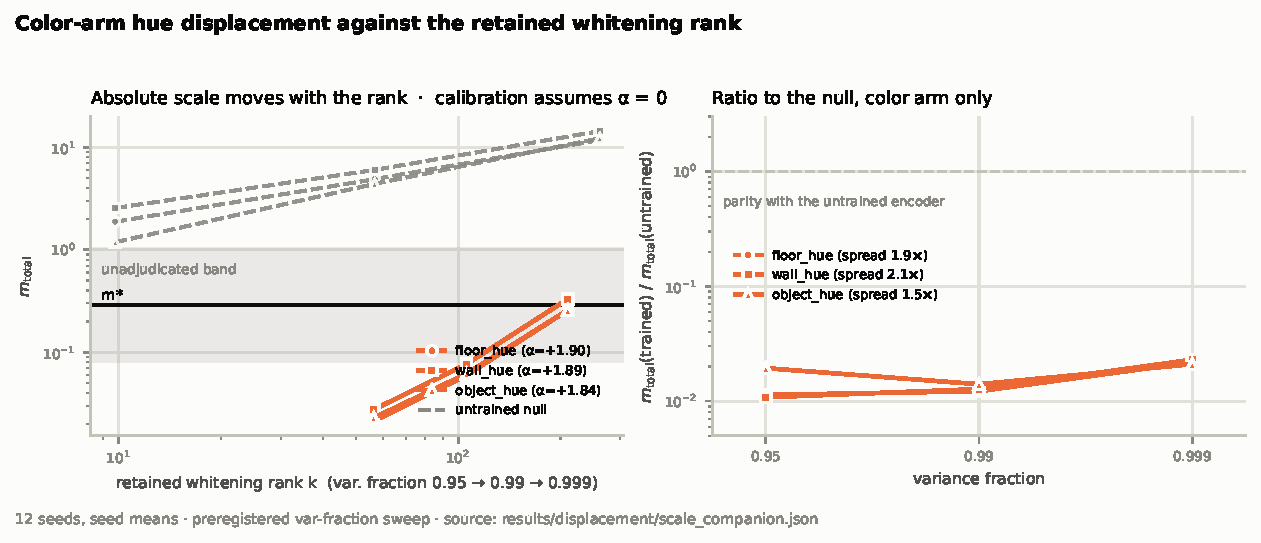
\includegraphics[width=0.92\linewidth]{figures/displacement_rank.pdf}
\caption{Color-arm displacement across the preregistered variance-fraction sweep. Left:
$m_{\mathrm{total}}$ for hue (orange) and the untrained null (gray dashed), with $m^{*}$ and the
unadjudicated band. Right: matched trained-to-untrained ratios. Absolute displacement grows with
rank, whereas the ratio remains $1.6$ to $2.0$ orders of magnitude below parity.}
\label{fig:disprank}
\end{figure}

\subsection*{Cross-arm comparison at unlike rank}
At the primary fraction, trained ranks are $435.5$ in Control-aug, $105.8$ in color and $64.0$ in
crop-plus-color, against a shared untrained rank of $56.8$; the two Control-aug roles have
attainable scales $\sqrt{2k}$ of $29.5$ and $10.7$. Fitted rank exponents across the sweep run from
$+0.54$ to $+1.90$.

Two corrections bound the contrast. Applying the color-arm hue exponent reduces the raw $295$-fold
floor-hue contrast to about $20$, and conservative corrections leave a $20$--$23$ separation across
all three hues. Using the Control-aug exponent leaves a gap about five times larger, so we report
the smaller estimate. Normalizing each role by its own $m_{\mathrm{ctx}}$ instead changes the
Control-aug hue values from $17.63$ versus $4.89$ to $0.655$ versus $0.518$, and the
control-to-color separation from $295$--$342$ to $154$--$182$, about $2.2$ orders of magnitude.
Floor and object hue then sit at $0.75$ and $0.77$ of the lower band edge and wall hue at $0.959$,
within $4.1\%$, which explains its seven-to-five split.

Because the fixture has lower rank than the measured fields, its threshold makes movement easier to
declare, the conservative direction Section~\ref{sec:limitations} states. Extrapolating an exact
correction from ranks $56$--$210$ to rank 1 would be unjustified.

\subsection*{Which companion survives the sweep}
The stability of the trained-to-null ratio is a color-arm property, and having swept all three arms
we can say where each companion holds (Table~\ref{tab:sweepstab}). In the control and
position arms the ordering inverts: $m_{\mathrm{total}}$ is the stable statistic and the ratio is
the unstable one, by up to a factor of $105$, and it crosses parity. Control-aug
scale runs $10.35$, $1.64$ and $0.53$ across the sweep and orientation runs $11.40$, $1.95$ and
$0.63$, so at $0.999$ the trained encoder displaces those two factors \emph{less} than the untrained
null does. Position-arm targeted factors cross earlier, at $11.00$, $0.47$ and $0.28$ on $x$ and
$11.19$, $0.46$ and $0.28$ on $y$. Within-role ratios cross as well, with Control-aug floor hue at
$1.62$, $0.88$ and $0.78$.

\begin{table}[tb]
\centering
\caption{Which companion survives the preregistered variance-fraction sweep, per arm. Each entry is
the ratio of the largest to the smallest value across variance fractions $0.95$, $0.99$ and $0.999$,
over the arm's targeted factors for the color row and over all its factors otherwise. The
trained-to-null ratio is stable on the color arm and least stable in the other two, so we
co-report it per arm.}
\label{tab:sweepstab}
\small
\begin{tabular}{l cc l}
\toprule
Arm & $m_{\mathrm{total}}$ spread & ratio-to-null spread & stable companion \\
\midrule
Color (hue factors) & $11.2$--$12.1$ & $1.5$--$2.1$ & ratio to null \\
Control-aug          & $1.4$--$1.6$   & $4.0$--$19.4$ & $m_{\mathrm{total}}$ \\
Position             & $2.1$--$4.4$   & $14.6$--$105.3$ & $m_{\mathrm{total}}$ \\
\bottomrule
\end{tabular}
\end{table}

A moving denominator explains it. Whitening the untrained role retains whatever rank that role's own
spectrum gives, and on dSprites the untrained rank swings
from $2.3$ to $44.7$ to $316.5$ across the sweep, a factor of $136$, while the trained rank moves
from $92.8$ to $183.5$ to $377.2$, a factor of $4$. A ratio whose denominator moves $136$-fold
normalizes nothing. The pattern is milder in Control-aug, at $9.8$, $56.8$ and $260.9$
untrained against $283.5$, $435.5$ and $502.4$ trained. The color arm's stability is the coincidence
of its two roles moving together, not a property of the statistic.

Both ends of the dSprites sweep are numerically uncomfortable. Retaining $2.3$ of
$512$ directions, as the untrained role does at $0.95$, is degenerate, and the trained role's
condition number at $0.999$ reaches $5984$ against $410$ in Control-aug. Our preregistered
primary at $0.99$ lies in the well-behaved middle of that range, which nothing in the calibration
anticipated, so the choice of fraction is not validated by it.

\subsection*{The control and position arms}
We ran the preregistered variance-fraction sensitivity on these two arms as well, so every arm's
reading spans three fractions. In Control-aug the verdict does not move:
six factors by twelve seeds by three fractions is $216$ seed-level verdicts and every one is
\emph{moves}. Orientation makes the tightest approach to the band at each fraction, at $2.34$,
$3.25$ and $3.66$ times its upper edge. Those three files share
the context seed, the calibration source, the band, and the same twelve trained and twelve untrained
roles, and differ only in the variance fraction.

In the position arm displacement also stays above the band across the sweep, narrowly at the low
end. At $0.99$ and $0.999$ all five factors on all twelve seeds are \emph{moves}; at
$0.95$, $59$ of $60$ are, with one seed's $x$ position falling into the band. Targeted factors
sit at $1.89$ and $1.87$ times the band's upper edge at $0.99$ and at $4.64$ times it at $0.999$,
and at $0.95$ they land on the edge itself: that seed measured $1.0407$ on $x$, just below the edge
of
$1.0445$, and $1.0445$ on $y$, above it by $3.30 \times 10^{-5}$. Section~\ref{sec:limitations}
takes that boundary case up.

The position arm therefore reads intermediate on both instruments: its targeted factors close
partially on the closure fraction, at $+0.164$ and $+0.147$, and displace at $28\%$ to $47\%$ of the
untrained null while staying above the band at the primary fraction and above. Those two
instruments share no failure mode, so that reading is a property of the arm.


\section{The excluded and exploratory arms}
\label{app:exploratory}
None of the three exploratory arms below enters a confirmatory family or any multiple-comparison
correction. Sections~\ref{sec:gate} and~\ref{sec:limitations} state what each supports.

\begin{figure}[tb]
\centering
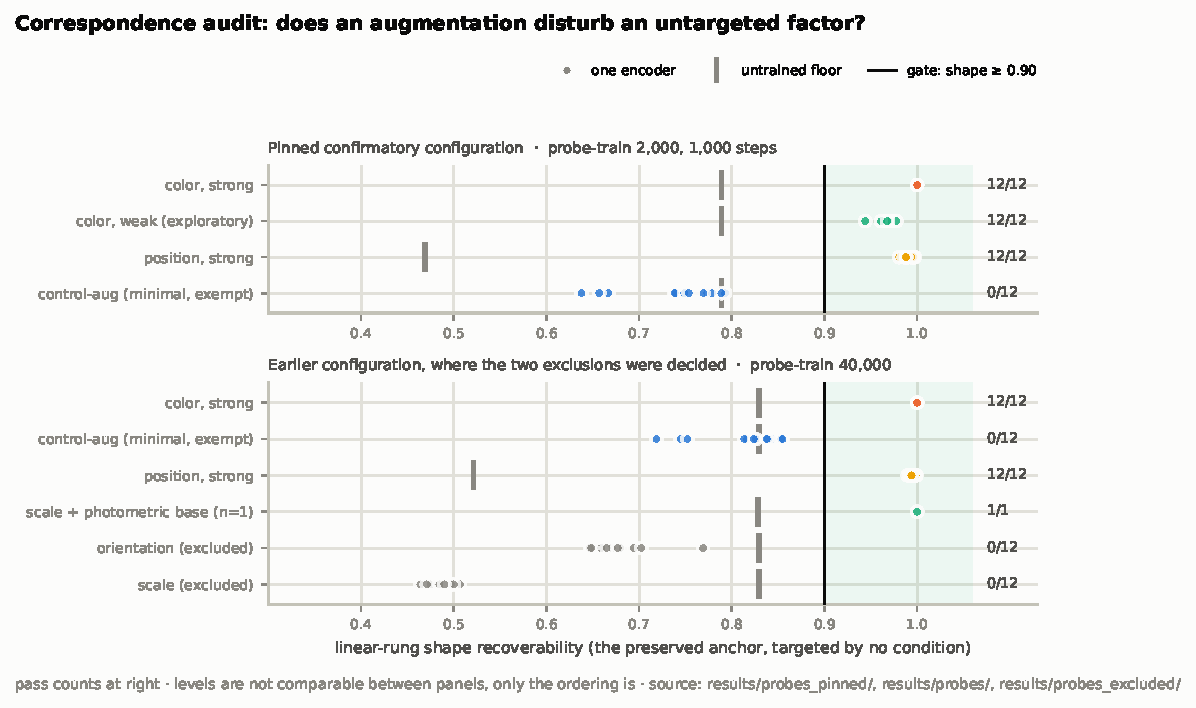
\includegraphics[width=0.92\linewidth]{figures/gate_audit.pdf}
\caption{Correspondence audit by encoder. Markers show linear-rung shape recoverability, gray ticks
each cell's untrained floor, and the vertical line the $0.90$ gate. The panels use different probe
configurations, so only within-panel ordering is comparable. Control-aug is exempt under amendment
A2.}
\label{fig:gate}
\end{figure}

\subsection*{Optimization and collapse diagnostics}
These do not explain the two correspondence failures. Orientation-arm encoders have feature standard
deviation $0.47$ and effective rank $235$, exceeding
the values for color ($0.205$, $118$) and position ($0.202$, $153$); collapse would reduce
both quantities.

\subsection*{The scale-recipe control and the weak-color arm}
Adding a canonical
photometric base to the same scale transform changed the shape anchor from $0.4833$ across twelve
seeds
(range $0.4640$ to $0.5066$, standard deviation $0.0132$) to $1.0000$, and the gate from $0/12$ to
$1/1$ on both criteria. That one-seed pilot exceeds the maximum of the twelve-seed comparison by
$0.4934$, equivalent to $37$ standard deviations or $11.6$ observed ranges. These are descriptive
distances. Its manipulation check reduces object-hue recoverability to $0.0217$ against a random
floor of $0.8871$. It changes color jitter and random grayscale together, so it is
exploratory evidence only.

Our weak-color arm bears on the same mechanism from the other side. Shapes3D is
$10\times10\times10$ in hue against a geometry grid of $480$, so the hue triple identifies an image
one in a thousand and NT-Xent is solvable from hue alone. On that account any photometric
augmentation should close the shortcut, with limited dependence on magnitude. Weak color applies one
quarter of the jitter and omits grayscale, yet clears the gate on all twelve seeds at
$0.9680$, with every weak seed below every strong seed. Strong to weak costs $0.0320$ of anchor and
weak to control costs $0.2310$. A monotone direction appears, but the steps are $7.2$ to $1$ apart,
consistent with a threshold-like response over the two tested strengths. Adding color jitter
restored the anchor in both exploratory controls, which partially separates the recipe pilot's
coupled changes.

\subsection*{The crop-plus-color pilot}
This pilot fills the cell that carries both a crop and color jitter. Beyond adding the crop it
changes crop scale to $0.3$--$1.0$, adds horizontal flip, uses photometric strengths $0.4$ and hue
$0.1$ against $0.5$, and trains for $100$ epochs against $50$, on one seed and in no
confirmatory family.

Its deepest-rung hue scores are $0.810$, $0.911$ and $0.705$ and its permuted-task scores
are $0.633$, $0.914$ and $0.360$. Displacement classifies all three hues as moving, at
$2.23$, $4.97$ and $3.59$ against $0.060$, $0.077$ and $0.062$ in color; a rank difference of $64.0$
against $105.8$ predicts about a $2.6$-fold change, far smaller than the observed
$37$--$65$-fold gap. Its closure fractions, $+0.426$, $+0.566$ and $+0.215$, lie $34.6\%$--$53.5\%$
of the way from Control-aug to color, while linear deficits move only $5.0\%$--$9.6\%$ of that
distance. These results associate cropping with whether hue survives and color jitter with
how much of the linear deficit closes; they do not identify either causal effect.

Two observations constrain alternative explanations. Our twelve-seed weak-color arm also uses hue
$0.1$ without a crop and yields deepest-rung hue scores $-0.104$, $-0.114$ and $-0.189$, with
closure fractions $-0.161$, $-0.205$ and $-0.272$, while the pilot applies stronger brightness,
contrast and saturation ($0.4$ versus $0.2$) plus grayscale and still retains hue. Longer
training does not readily explain the factor-specific pattern either: weak-color recovers non-hue
factors at $0.984$ and hue at $-0.136$ (gap $1.120$), while crop-plus-color gives $0.959$ and
$0.809$ (gap $0.150$). At one seed, both alternatives stay open, and a twelve-seed crop-plus-color
arm is the needed augmentation follow-up.

\section{Additional limitations}
\label{app:limits}
\subsection*{Affine stability of the whitener}
Whitening is exactly stable under orthogonal maps and only approximately stable under general
invertible maps. At width $64$, random invertible maps change $m_{\mathrm{total}}$ by a mean
$17.2\%$ at fraction $0.95$, $13.4\%$ at $0.99$, $6.7\%$ at $0.999$ and $0.25\%$ at full rank.
Projecting out near-null eigenvectors avoids the thousand-fold amplification seen with eigenvalue
flooring. We tested this property for displacement only. Establishing affine stability for the
closure fraction would require refitting every probe on reparameterized representations, beyond
the present experiment \citep{lee2026shallow}.

\subsection*{Precision of the displacement verdicts}
At variance fraction $0.95$, one position seed lies on the band boundary: $x=1.0407$ is
unadjudicated, while $y=1.0445$ is moving by $3.30 \times 10^{-5}$. Both intervals cross the edge.
The preregistered point-estimate rule changes one of $60$ seed verdicts at this fraction and none at
$0.99$ or $0.999$. We calibrated the threshold on Shapes3D and transferred it unchanged to dSprites.

We exclude the monotonicity diagnostic from verdicts. Its mean fraction is $0.00$ for every hue
and position readout and at most $0.294$ elsewhere, including factors classified as moving. It
examines signs along one leading singular direction, whereas $m_{\mathrm{total}}$ averages norms
over effective ranks $45.6$--$353.3$; the diagnostic is poorly matched to these multidirectional
fields.

\section{Preregistration and amendment trail}
\label{app:amendments}
We locked the hypotheses, their decision rules and every operational definition of
Section~\ref{sec:defs} on 2026-06-28, following an independent methods review, and changed them
afterwards only through the fifteen dated amendments in Table~\ref{tab:amendments}. We ran
the confirmatory statistics, and broke the blind, on 2026-08-24. The last amendment is dated
2026-08-19, so every entry below precedes the first sight of a confirmatory verdict. Each amendment
in the frozen document carries an unblinding-status paragraph recording what had and had not been
computed when it was filed, and that paragraph, more than the date, is the substance of the claim.
That full document is part of the repository described in Appendix~\ref{app:artifacts}.

Amendment A6 appears between A9 and A10 in that document and in date order here, because entries are
appended or inserted and never rewritten; A6's
own text is unchanged since our version history first records it on 2026-07-29, the day after the
date it bears. Position matters here because A6 pre-commits the scale-arm decision rule
that A7 executes, and its unblinding-status paragraph records that the bounded scale retrain the
rule judges had not been run when the rule was filed. The
predecessor configuration had been inspected, which we state explicitly: an
earlier unbounded $(0.6, 1.4)$ scale arm's shape anchor was inspected on three seeds eight days
before A6, reading $0.383$ to $0.390$ against an untrained floor near $0.83$, and that reading is
why the augmentation was bounded. It reads the untargeted anchor alone, on an arm that is not the
one A6's rule judges. Those values come from that run's log, since
its encoders are not part of the realized grid and we do
not release them.

{\footnotesize
\begin{longtable}{@{}llp{10.4cm}@{}}
\caption{The fifteen dated amendments to the preregistration frozen on 2026-06-28. The confirmatory
statistics were run on 2026-08-24, after the last of them.}
\label{tab:amendments} \\
\toprule
 & Date & What it changed \\
\midrule
\endfirsthead
\multicolumn{3}{@{}l}{\textit{Table \ref{tab:amendments}, continued.}} \\
\toprule
 & Date & What it changed \\
\midrule
\endhead
A1  & 2026-07-13 & Grid curtailed to the strong cross-section. H4's widening rule becomes
inevaluable at one strength, so H4 is reduced to its sign component and labeled descriptive.
Flip-count uncertainty and absolute recoverability levels added to reporting. \\
A2  & 2026-07-14 & The encoder-quality gate is scoped to treatment arms, exempting the
minimal-augmentation control on its preregistered design role. No decision rule changes. \\
A3  & 2026-07-15 & The dSprites orientation readout leaves every confirmatory family as
non-identifiable from pixels, and is retained as a labeled diagnostic. \\
A4  & 2026-07-16 & Headroom, one minus the random-encoder floor, is reported per factor and rung; a
raw-pixel reference ladder is added as a diagnostic; each arm's reading is pinned to the
arm-to-factor map instead of the condition's name. Additive reporting only. \\
A5  & 2026-07-28 & The Shapes3D orientation arm is excluded, on the shape gate as it then stood
and on the argument that in-plane rotation and camera azimuth are different group actions. Under
A8's later three-valued gate that arm is indeterminate, so the group-action argument is the
ground we report. \\
A6  & 2026-07-28 & The null-saturation gate on H3 and the flip count; the capacity-axis validity
check; the maximal-Holm-family disclosure; and the scale-arm decision rule, pre-committed with its
threshold before the retrain it would judge was run. \\
A7  & 2026-08-07 & The scale arm is excluded, executing A6's pre-committed rule at $0/12$. The
realized grid is frozen at three cells and no further cell may be removed for any reason. The
divergence of the trained scale transform from the preregistered random-resized-crop variant is
disclosed. \\
A8  & 2026-08-07 & Four metric defects repaired: $\epsG$ becomes a null quantile instead of a
bootstrap interval of a quantity identically zero, the random-label control is made learnable, a
headroom-normalized co-primary is added, and H4 gains a matched untrained projector floor. The
quality gate becomes three-valued. Both rule changes move against the study's hypotheses. \\
A9  & 2026-08-11 & The probe optimization budget is pinned in gradient steps instead of epochs, so
effort is fixed across the ladder and across the probe-train sweep. \\
A10 & 2026-08-12 & Probe targets are standardized, voiding every continuous readout computed before
this date. The primary invariance boolean becomes two-sided, keyed on the deficit direction, so a
readout sitting at the untrained floor is recovered instead of invariant. \\
A11 & 2026-08-13 & The counterfactual displacement spectrum, a destruction certificate and the
displacement-to-capacity-gap link test are preregistered, before the instrument had ever run. \\
A12 & 2026-08-13 & Two parts of A11 are retired the same day: its certificate was relative and, on a
synthetic fixture, certified destruction of a perfectly decodable factor, and its energy-fraction
statistic does not bound linear decodability. \\
A13 & 2026-08-13 & The link test gains a per-seed statistic; the closure fraction $\kappa$ is
defined as a supporting diagnostic; an input-side control admitted as ground truth, and an
external-encoder check, are added. \\
A14 & 2026-08-16 & No swept configuration clears A10's all-factor headroom veto, so the veto becomes
a per-readout reporting requirement and the pin stands. Discloses, pre-verdict, that every targeted
factor of every realized arm is null-saturated. \\
A15 & 2026-08-19 & Four certificate defects repaired before the instrument's first run: the
artifacts still declared A12's retired rule, the live rule had no constant, the reduction control it
would have treated as ground truth leaks measurably, and the whitener amplified near-null
directions. $m^{*}$ is calibrated, the verdict is renamed to $\epsilon$-destruction at a stated
resolution, and the variance-fraction sweep becomes a preregistered sensitivity. The last
amendment. \\
\bottomrule
\end{longtable}
}

\textbf{What was removed, and on what grounds.} Three amendments removed something and their
grounds differ. A3 removed one readout everywhere, on an identifiability argument about pixels that
inspects no measured value: distinct latent orientations of a $90^\circ$-periodic square map to
identical images, so any invariance verdict there would be vacuous. A5 and A7 each removed an arm,
and neither decision inspected a targeted-factor result. Every augmentation in the study leaves
shape untargeted, so the gate that evaluates it is orthogonal by construction to every
targeted-factor hypothesis. As the gate now stands, exactly one exclusion rests on its verdict: A7
removed the scale arm on the \texttt{FAIL-DESTROYED} branch, executing a rule pre-committed ten days
earlier in A6 with its threshold fixed before the retrain it would judge. A5 removed the orientation
arm while the gate was still two-valued and cited it; A8 then made the gate three-valued, under
which that arm is indeterminate and no exclusion follows. What survives there is the group-action
argument A5 gives alongside, which no measurement could reach, and we report the gate's reading
beside it. After A7 no cell may leave the confirmatory families for any reason, so a fourth
exclusion would have re-scoped the study as a negative result about augmentation-to-factor
correspondence.

Every removal narrows the Holm family and so lightens the correction burden on the survivors, which
is why we report the designed family beside the realized one throughout.

\textbf{The maximal Holm family.} A6 required a sensitivity analysis over all five originally
designed cells. Of its
forty-three pairs, twenty-nine survive, including every one of the twelve realized-family results.
Ten have the exact two-sided Wilcoxon floor at twelve seeds, $4.88\times10^{-4}$, and survive any
family of up to $102$ tests. The other two have Holm-adjusted $p=0.0415$ at $\alpha=0.05$ after the
twenty comparisons from the excluded cells are added, and that margin depends on those added pairs:
treating all twenty as uninformative moves the two to a Holm-adjusted
$0.0806$, while the ten at the floor hold. Those diagnostic cells use the earlier probe
configuration voided by A10 and contribute only to this check. Every H2 survivor predates the
narrowing, and both excluded conditions stay excluded.

\textbf{Two rules moved against the study's hypotheses.} A8 replaced $\epsG$ with a null quantile,
raising it more than tenfold over the estimator it replaced and so making invariance easier to
declare, and it made the quality gate harder to fail by requiring a non-closing deficit before an
arm may be excluded. A10 voided every continuous readout the study had computed to that point, its
own included, and moved the primary invariance boolean to the deficit direction. The color arm's
scale readout at the earlier configuration was $-1.653$, against $0.999$ at the pinned
configuration, and remains available solely as a diagnostic. A10 is the rule
under which H3 is refuted and under which the frozen one-sided reading disagrees on exactly one
readout. Neither rule narrowed a family nor removed a cell, and we report both with the frozen
variant beside them.

\textbf{Certificate amendment sequence.} A11 preregistered the certificate while
\texttt{results/displacement/} did not yet exist, and the loader refuses a trained checkpoint unless
that amendment is named on the command line. A12 retired its verdict rule the same day, and A15
fixed the four remaining defects, renamed what a verdict supports to $\epsilon$-destruction at a
stated resolution, published the calibration fixing that resolution, and reserved a band of factor
$13.1$ inside which the instrument returns no verdict at all. The rule
went through three versions in six days, A11 and A12 on 2026-08-13 and A15 on 2026-08-19,
all before the instrument had scored a trained checkpoint, and its net effect is strictly weaker
than what A11 and A12 allowed.

\textbf{The one change after the trail: the promotion of $\kappa$.} Every amendment predates the
unblinding; the weight this paper puts on $\kappa$ does not. A13 introduced the closure fraction
on 2026-08-13 as a supporting diagnostic, and this paper now organizes its abstract, introduction
and results around it. That reweighting happened after 2026-08-24, when the preregistered program
returned H1
confirmed almost entirely on the untreated arm, H3 refuted by the instrument's own ceiling, and both
H4's widening component and the displacement-to-capacity link test not evaluable. Our organizing
frame is therefore post-hoc with respect to the lock, and two things constrain what it could be
made to say. We fixed $\kappa$'s definition, its decision-free construction and the bootstrap that
produces its intervals in A13, before computing it on any cell, so the statistic was not shaped to
the result. And Section~\ref{sec:prereg} reports all four hypotheses, the flip count and its six
variants under their frozen rules whatever they returned, so the reframing adds an emphasis without
replacing a verdict.

\textbf{The trail stops before the verdicts.} A15 is the last amendment. Confirmatory statistics ran
five days later and no amendment is dated after that. Defects we identified afterwards we report as
limitations in Section~\ref{sec:limitations}, including the variance-fraction
sensitivity that weakens the certificate's headline verdict and the $m_{\mathrm{shared}}$
re-scoring, which is labeled post-hoc and is not shipped as the certificate's scale. We added two
arms after that date and neither is an amendment: we probed the weak-color and scale-recipe cells on
2026-09-05, after the blind broke. We trained the crop-plus-color cell on 2026-07-04 and
probed it on 2026-09-07, so its selection into this paper is post-unblinding as well. We label all
three exploratory wherever they appear, with their sample sizes and confounds attached, and none
enters a confirmatory family or any multiple-comparison correction.

\end{document}
